
\makeatletter
\@ifundefined{standalonetrue}{\newif\ifstandalone}{}
\@ifundefined{section}{\standalonetrue}{\standalonefalse}
\makeatother
\ifstandalone
\documentclass{report}

\usepackage{textcase}
%\usepackage{hyperref}
%\hypersetup{breaklinks=true}


% Added packages
\usepackage[usenames]{color}
\usepackage{amsfonts, amsmath, amssymb, graphics}

% NOTE: bibentry MUST appear before the hyperref or build will fail
\usepackage{bibentry}
\nobibliography*
\usepackage[square,sort,comma,numbers]{natbib}
  
\usepackage{float}
\usepackage[
	hidelinks,%
    %hyperindex=true,		% Make numbers of index links as well
   	backref=page, 		% Provide page listing where refs occur in the bibliography
	%breaklinks=true,
    %colorlinks,%
    %citecolor=green,%
    %filecolor=blue,%
    %linkcolor=red,%
    %urlcolor=red, 
]{hyperref}

\usepackage{dsfont}
%%%% USEPACKAGES for MACROS %%%%%
\usepackage{algpseudocode}
\usepackage[chapter]{algorithm}
%\usepackage{caption}
\usepackage{subcaption}
\usepackage{url}

\usepackage{array}
\usepackage{arydshln}
\usepackage{multirow}
\usepackage{multicol}
%\usepackage[section]{placeins}

\usepackage[usenames,dvipsnames]{color}
%\usepackage[english]{babel}
\usepackage{tabularx}
\usepackage{soul}
\usepackage{xparse}
\usepackage{listings}
%\usepackage[normalem]{ulem}



%%%%%%%%%%%%%%%
% Show a list of items "todo" or "done" 
% USAGE: 
% \begin{todolist} 
% 	\todo Something not finished
% 	\done Something finished
% \end{todolist} 
\newenvironment{todolist}{%
  \begin{list}{}{}% whatever you want the list to be
  \let\olditem\item
  \renewcommand\item{\olditem \textcolor{red}{(TODO)}: }
  \newcommand\todo{\olditem \textcolor{red}{(TODO)}: }
   \newcommand\done{\olditem \textcolor{ForestGreen}{(DONE)}: }
}{%
  \end{list}
} 
%%%%%%%%%%%%%%%

%%%%%%%%%%%%%%%
% Show a Author's Note
% USAGE: 
% \incomplete[Optional footnote message to further clarify note]{The text which is currently not finished}
\DeclareDocumentCommand \incomplete{ o m }
{%
\IfNoValueTF {#1}
{\textcolor{red}{Incomplete: \ul{#2}}} 
{\textcolor{red}{Incomplete: \ul{#2}}\footnote{Comment: #1}}%
}
%%%%%%%%%%%%%%%



%%%%%%%%%%%%%%%
% Show a Author's Note
% USAGE: 
% \authnote[Optional footnote message to further clarify note]{The note to your readers}
\DeclareDocumentCommand \authnote { o m }
{%
\IfNoValueTF {#1}
{\textcolor{blue}{Author's Note: \ul{#2}}} 
{\textcolor{blue}{Author's Note: \ul{#2}}\footnote{Comment: #1}}%
}
%%%%%%%%%%%%%%%



%%%%%%%%%%%%%%%
% Strike out text that doesn't belong in the paper
% USAGE: 
% \strike[Optional footnote to state why it doesn't belong]{Text to strike out}
\DeclareDocumentCommand \strike { o m }
{%
\setstcolor{Red}
\IfNoValueTF {#1}
{\textcolor{Gray}{\st{#2}}} 
{\textcolor{Gray}{\st{#2}}\footnote{Comment: #1}}%
}
%%%%%%%%%%%%%%%

\definecolor{light-gray}{gray}{0.95}

\newcommand{\cbox}[3]{
\ \\
\fcolorbox{#1}{#2}{
\parbox{\textwidth}{
#3
}
}
}

% Setup an environment similar to verbatim but which will highlight any bash commands we have
\lstnewenvironment{unixcmds}[0]
{
%\lstset{language=bash,frame=shadowbox,rulesepcolor=\color{blue}}
\lstset{ %
language=sh,		% Language
basicstyle=\ttfamily,
backgroundcolor=\color{light-gray}, 
rulecolor=\color{blue},
%frame=tb, 
columns=fullflexible,
%framexrightmargin=-.2\textwidth,
linewidth=0.8\textwidth,
breaklines=true,
%prebreak=/, 
  prebreak = \raisebox{0ex}[0ex][0ex]{\ensuremath{\hookleftarrow}},
%basicstyle=\footnotesize,       % the size of the fonts that are used for the code
%numbers=left,                   % where to put the line-numbers
%numberstyle=\footnotesize,      % the size of the fonts that are used for the line-numbers
%stepnumber=2,                   % the step between two line-numbers. If it's 1 each line 
                                % will be numbered
%numbersep=5pt,                  % how far the line-numbers are from the code
showspaces=false,               % show spaces adding particular underscores
showstringspaces=false,         % underline spaces within strings
showtabs=false,                 % show tabs within strings adding particular underscores
frame=single,	                % adds a frame around the code
tabsize=2,	                % sets default tabsize to 2 spaces
captionpos=b,                   % sets the caption-position to bottom
breakatwhitespace=false,        % sets if automatic breaks should only happen at whitespace
}
} { }

% Setup an environment similar to verbatim but which will highlight any bash commands we have
\lstnewenvironment{cppcode}[1]
{
%\lstset{language=bash,frame=shadowbox,rulesepcolor=\color{blue}}
\lstset{ %
	backgroundcolor=\color{light-gray}, 
	rulecolor=\color[rgb]{0.133,0.545,0.133},
	tabsize=4,
	language=[GNU]C++,
%	basicstyle=\ttfamily,
        basicstyle=\scriptsize,
        upquote=true,
        aboveskip={1.5\baselineskip},
        columns=fullflexible,
        %framexrightmargin=-.1\textwidth,
       %framexleftmargin=6mm,
        showstringspaces=false,
        extendedchars=true,
        breaklines=true,
        prebreak = \raisebox{0ex}[0ex][0ex]{\ensuremath{\hookleftarrow}},
        frame=single,
        showtabs=false,
        showspaces=false,
        showstringspaces=false,
        numbers=left,                   % where to put the line-numbers
	numberstyle=\footnotesize,      % the size of the fonts that are used for the line-numbers
	stepnumber=4,                   % the step between two line-numbers. If it's 1 each line 
                                % will be numbered
	firstnumber=#1,
         numbersep=5pt,                  % how far the line-numbers are from the code
        identifierstyle=\ttfamily,
        keywordstyle=\color[rgb]{0,0,1},
        commentstyle=\color[rgb]{0.133,0.545,0.133},
        stringstyle=\color[rgb]{0.627,0.126,0.941},
}
} { }

% Setup an environment similar to verbatim but which will highlight any bash commands we have
\lstnewenvironment{mcode}[1]
{
\lstset{ %
	backgroundcolor=\color{light-gray}, 
	rulecolor=\color[rgb]{0.133,0.545,0.133},
	tabsize=4,
	language=Matlab,
%	basicstyle=\ttfamily,
        basicstyle=\scriptsize,
        upquote=true,
        aboveskip={1.5\baselineskip},
        columns=fullflexible,
        %framexrightmargin=-.1\textwidth,
       %framexleftmargin=6mm,
        showstringspaces=false,
        extendedchars=true,
        breaklines=true,
        prebreak = \raisebox{0ex}[0ex][0ex]{\ensuremath{\hookleftarrow}},
        frame=single,
        showtabs=false,
        showspaces=false,
        showstringspaces=false,
        numbers=left,                   % where to put the line-numbers
	numberstyle=\footnotesize,      % the size of the fonts that are used for the line-numbers
	stepnumber=4,                   % the step between two line-numbers. If it's 1 each line 
                                % will be numbered
	firstnumber=#1,
         numbersep=5pt,                  % how far the line-numbers are from the code
        identifierstyle=\ttfamily,
        keywordstyle=\color[rgb]{0,0,1},
        commentstyle=\color[rgb]{0.133,0.545,0.133},
        stringstyle=\color[rgb]{0.627,0.126,0.941},
}
} { }

\newcommand{\inputmcode}[1]{%
\lstset{ %
	backgroundcolor=\color{light-gray},  %
	rulecolor=\color[rgb]{0.133,0.545,0.133}, %
	tabsize=4, %
	language=Matlab, %
%	basicstyle=\ttfamily,
        basicstyle=\scriptsize, %
        %        upquote=true,
        aboveskip={1.5\baselineskip}, %
        columns=fullflexible, %
        %framexrightmargin=-.1\textwidth,
       %framexleftmargin=6mm,
        showstringspaces=false, %
        extendedchars=true, %
        breaklines=true, %
        prebreak = \raisebox{0ex}[0ex][0ex]{\ensuremath{\hookleftarrow}}, %
        frame=single, %
        showtabs=false, %
        showspaces=false, %
        showstringspaces=false,%
        numbers=left,                   % where to put the line-numbers
	numberstyle=\footnotesize,      % the size of the fonts that are used for the line-numbers
	stepnumber=4,                   % the step between two line-numbers. If it's 1 each line 
                                % will be numbered
         numbersep=5pt,                  % how far the line-numbers are from the code
        identifierstyle=\ttfamily, %
        keywordstyle=\color[rgb]{0,0,1}, %
        commentstyle=\color[rgb]{0.133,0.545,0.133}, %
        stringstyle=\color[rgb]{0.627,0.126,0.941} %
}
\lstinputlisting{#1}%
}

%\lstset{ %
%	backgroundcolor=\color{light-gray}, 
%	rulecolor=\color[rgb]{0.133,0.545,0.133},
%	tabsize=4,
%	language=Matlab,
%%	basicstyle=\ttfamily,
%        basicstyle=\scriptsize,
%        upquote=true,
%        aboveskip={1.5\baselineskip},
%        columns=fullflexible,
%        %framexrightmargin=-.1\textwidth,
%       %framexleftmargin=6mm,
%        showstringspaces=false,
%        extendedchars=true,
%        breaklines=true,
%        prebreak = \raisebox{0ex}[0ex][0ex]{\ensuremath{\hookleftarrow}},
%        frame=single,
%        showtabs=false,
%        showspaces=false,
%        showstringspaces=false,
%        numbers=left,                   % where to put the line-numbers
%	numberstyle=\footnotesize,      % the size of the fonts that are used for the line-numbers
%	stepnumber=4,                   % the step between two line-numbers. If it's 1 each line 
%                                % will be numbered
%	firstnumber=#1,
%         numbersep=5pt,                  % how far the line-numbers are from the code
%        identifierstyle=\ttfamily,
%        keywordstyle=\color[rgb]{0,0,1},
%        commentstyle=\color[rgb]{0.133,0.545,0.133},
%        stringstyle=\color[rgb]{0.627,0.126,0.941},
%}


\newcommand{\Laplacian}[1]{\nabla^2 #1}

% set of all nodes received and contained on GPU
\newcommand{\setAllNodes}[0]{\mathcal{G}}
% set of stencil centers on GPU
\newcommand{\setCenters}[0]{\mathcal{Q}}
% set of stencil centers with nodes in \setDepend
\newcommand{\setBoundary}[0]{\mathcal{B}}
% set of nodes received by other GPUs
\newcommand{\setDepend}[0]{\mathcal{R}}
% set of nodes sent to other GPUs
\newcommand{\setProvide}[0]{\mathcal{O}}


\newcommand{\toprule}[0]{\hline}
\newcommand{\midrule}[0]{\hline\hline}
\newcommand{\bottomrule}[0]{\hline}

\newcolumntype{C}{>{\centering\arraybackslash}b{1in}}
\newcolumntype{L}{>{\flushleft\arraybackslash}b{1.5in}}
\newcolumntype{R}{>{\flushright\arraybackslash}b{1.5in}}
\newcolumntype{D}{>{\flushright\arraybackslash}b{2.0in}}
\newcolumntype{E}{>{\flushright\arraybackslash}b{1.0in}}

\DeclareSymbolFont{AMSb}{U}{msb}{m}{n}
\DeclareMathSymbol{\N}{\mathbin}{AMSb}{"4E}
\DeclareMathSymbol{\Z}{\mathbin}{AMSb}{"5A}
\DeclareMathSymbol{\R}{\mathbin}{AMSb}{"52}
\DeclareMathSymbol{\Q}{\mathbin}{AMSb}{"51}
\DeclareMathSymbol{\PP}{\mathbin}{AMSb}{"50}
\DeclareMathSymbol{\I}{\mathbin}{AMSb}{"49}
%\DeclareMathSymbol{\C}{\mathbin}{AMSb}{"43}

%%%%%% VECTOR NORM: %%%%%%%
\newcommand{\vectornorm}[1]{\left|\left|#1\right|\right|}
\newcommand{\vnorm}[1]{\left|\left|#1\right|\right|}
\newcommand{\by}[0]{\times}
\newcommand{\vect}[1]{\mathbf{#1}}
%\newcommand{\mat}[1]{\mathbf{#1}} 

%\renewcommand{\vec}[1]{ \textbf{#1} }
%%%%%%%%%%%%%%%%%%%%%%

%%%%%%% THM, COR, DEF %%%%%%%
%\newtheorem{theorem}{Theorem}[section]
%\newtheorem{lemma}[theorem]{Lemma}
%\newtheorem{proposition}[theorem]{Proposition}
%\newtheorem{corollary}[theorem]{Corollary}
%\newenvironment{proof}[1][Proof]{\begin{trivlist}
%\item[\hskip \labelsep {\bfseries #1}]}{\end{trivlist}}
%\newenvironment{definition}[1][Definition]{\begin{trivlist}
%\item[\hskip \labelsep {\bfseries #1}]}{\end{trivlist}}
%\newenvironment{example}[1][Example]{\begin{trivlist}
%\item[\hskip \labelsep {\bfseries #1}]}{\end{trivlist}}
%\newenvironment{remark}[1][Remark]{\begin{trivlist}
%\item[\hskip \labelsep {\bfseries #1}]}{\end{trivlist}}
%\newcommand{\qed}{\nobreak \ifvmode \relax \else
%      \ifdim\lastskip<1.5em \hskip-\lastskip
%      \hskip1.5em plus0em minus0.5em \fi \nobreak
%      \vrule height0.75em width0.5em depth0.25em\fi}
%%%%%%%%%%%%%%%%%%%%%%

%
%\usepackage[algochapter]{algorithm2e}
%\usepackage[usenames]{color}
% colors to show the corrections
\newcommand{\red}[1]{\textbf{\textcolor{red}{#1}}}
\newcommand{\blue}[1]{\textbf{\textcolor{blue}{#1}}}
\newcommand{\cyan}[1]{\textbf{\textcolor{cyan}{#1}}}
\newcommand{\green}[1]{\textbf{\textcolor{green}{#1}}}
\newcommand{\magenta}[1]{\textbf{\textcolor{magenta}{#1}}}
\newcommand{\orange}[1]{\textbf{\textcolor{orange}{#1}}}
%%%%%%%%%% DK DK
% comments between authors
\newcommand{\toall}[1]{\textbf{\green{@@@ All: #1 @@@}}}
\newcommand{\toevan}[1]{\textbf{\red{*** Evan: #1 ***}}}
%\newcommand{\toevan}[1]{}  % USE FOR FINAL VERSION
\newcommand{\toe}[1]{\textbf{\red{*** Evan: #1 ***}}}
\newcommand{\tog}[1]{\textbf{\blue{*** Gordon: #1 ***}}}
%\newcommand{\togordon}[1]{\textbf{\blue{*** Gordon: #1 ***}}}
\renewcommand{\ge}[3]{{\textcolor{blue}{*** \textbf{Gordon:}\strike{#1} #2 ***}}\red{(#3)}}
\renewcommand{\ge}[3]{{\textcolor{blue}{#2}}}
\renewcommand{\ge}[3]{{\textcolor{Red}{#2}}}
\newcommand{\eb}[3]{{\textcolor{Red}{*** \textbf{Evan:}\strike{#1} #2 ***}}\red{(#3)}}
\renewcommand{\eb}[3]{{{\textcolor{Red}{#2}}}}
%\def\ge#1#2#3{}{\textbf{\blue{*** Gordon: #2 ***}}}{(#3)}
\newcommand{\gee}[1]{{\bf{\blue{{\em #1}}}}}
\newcommand{\old}[1]{}
\newcommand{\del}[1]{***#1*** }



% \DeclareMathOperator{\Sample}{Sample}
%\let\vaccent=\v % rename builtin command \v{} to \vaccent{}
%\renewcommand{\vec}[1]{\ensuremath{\mathbf{#1}}} % for vectors
\newcommand{\gv}[1]{\ensuremath{\mbox{\boldmath$ #1 $}}} 
% for vectors of Greek letters
\newcommand{\uv}[1]{\ensuremath{\mathbf{\hat{#1}}}} % for unit vector
\newcommand{\abs}[1]{\left| #1 \right|} % for absolute value
\newcommand{\avg}[1]{\left< #1 \right>} % for average
\let\underdot=\d % rename builtin command \d{} to \underdot{}
\renewcommand{\d}[2]{\frac{d #1}{d #2}} % for derivatives
\newcommand{\dd}[2]{\frac{d^2 #1}{d #2^2}} % for double derivatives
\newcommand{\pd}[2]{\frac{\partial #1}{\partial #2}} 
% for partial derivatives
\newcommand{\pdd}[2]{\frac{\partial^2 #1}{\partial #2^2}} 
\newcommand{\pdda}[3]{\frac{\partial^2 #1}{\partial #2 \partial #3}} 
% for double partial derivatives
\newcommand{\pdc}[3]{\left( \frac{\partial #1}{\partial #2}
 \right)_{#3}} % for thermodynamic partial derivatives
\newcommand{\ket}[1]{\left| #1 \right>} % for Dirac bras
\newcommand{\bra}[1]{\left< #1 \right|} % for Dirac kets
\newcommand{\braket}[2]{\left< #1 \vphantom{#2} \right|
 \left. #2 \vphantom{#1} \right>} % for Dirac brackets
\newcommand{\matrixel}[3]{\left< #1 \vphantom{#2#3} \right|
 #2 \left| #3 \vphantom{#1#2} \right>} % for Dirac matrix elements
\newcommand{\grad}[1]{\gv{\nabla} #1} % for gradient
\let\divsymb=\div % rename builtin command \div to \divsymb
\renewcommand{\div}[1]{\gv{\nabla} \cdot #1} % for divergence
\newcommand{\curl}[1]{\gv{\nabla} \times #1} % for curl
\let\baraccent=\= % rename builtin command \= to \baraccent
\renewcommand{\=}[1]{\stackrel{#1}{=}} % for putting numbers above =
\newcommand{\diffop}[1]{\mathcal{L}#1}
\newcommand{\boundop}[1]{\mathcal{B}#1}
\newcommand{\rvec}[0]{{\bf r}}

\newcommand{\Interior}[0]{\Omega}
\newcommand{\domain}[0]{\Omega}
%\newcommand{\Boundary}[0]{\partial \Omega}
\newcommand{\Boundary}[0]{\Gamma}

\newcommand{\on}[1]{\hskip1.5em \textrm{ on } #1}

\newcommand{\gemm}{\texttt{GEMM}}
\newcommand{\trmm}{\texttt{TRMM}}
\newcommand{\gesvd}{\texttt{GESVD}}
\newcommand{\geqrf}{\texttt{GEQRF}}


\newcommand{\minitab}[2][l]{\begin{tabular}{#1}#2\end{tabular}}
\newcommand{\comm}[1]{\textcolor{red}{\textit{#1}}}

\newcommand{\nfrac}[2]{
\nicefrac{#1}{#2}
%\frac{#1}{#2}
}

\usepackage{xparse}
\usepackage{soul}


%%%%%%%%%%%%%%%
% Show a Author's Note
% USAGE: 
% \incomplete[Optional footnote message to further clarify note]{The text which is currently not finished}
\DeclareDocumentCommand \incomplete{ o m }
{%
\IfNoValueTF {#1}
{\textcolor{red}{Incomplete: \ul{#2}}} 
{\textcolor{red}{Incomplete: \ul{#2}}\footnote{Comment: #1}}%
}
%%%%%%%%%%%%%%%



%%%%%%%%%%%%%%%
% Show a Author's Note
% USAGE: 
% \authnote[Optional footnote message to further clarify note]{The note to your readers}
\DeclareDocumentCommand \authnote { o m }
{%
\IfNoValueTF {#1}
{\textcolor{blue}{Author's Note: \ul{#2}}} 
{\textcolor{blue}{Author's Note: \ul{#2}}\footnote{Comment: #1}}%
}
%%%%%%%%%%%%%%%



%%%%%%%%%%%%%%%
% Strike out text that doesn't belong in the paper
% USAGE: 
% \strike[Optional footnote to state why it doesn't belong]{Text to strike out}
\DeclareDocumentCommand \strike { o m }
{%
\setstcolor{red}
\IfNoValueTF {#1}
{\textcolor{Gray}{\st{#2}}} 
{\textcolor{Gray}{\st{#2}}\footnote{Comment: #1}}%
}
%%%%%%%%%%%%%%%



%
% colors to show the corrections
\newcommand{\red}[1]{\textbf{\textcolor{red}{#1}}}
\newcommand{\blue}[1]{\textbf{\textcolor{blue}{#1}}}
\newcommand{\cyan}[1]{\textbf{\textcolor{cyan}{#1}}}
\newcommand{\green}[1]{\textbf{\textcolor{green}{#1}}}
\newcommand{\magenta}[1]{\textbf{\textcolor{magenta}{#1}}}
\newcommand{\orange}[1]{\textbf{\textcolor{orange}{#1}}}
%%%%%%%%%% DK DK
% comments between authors
\newcommand{\toall}[1]{\textbf{\green{@@@ All: #1 @@@}}}
\newcommand{\toevan}[1]{\textbf{\red{*** Evan: #1 ***}}}
%\newcommand{\toevan}[1]{}  % USE FOR FINAL VERSION
\newcommand{\toe}[1]{\textbf{\red{*** Evan: #1 ***}}}
\newcommand{\tog}[1]{\textbf{\blue{*** Gordon: #1 ***}}}
%\newcommand{\togordon}[1]{\textbf{\blue{*** Gordon: #1 ***}}}
\renewcommand{\ge}[3]{{\textcolor{blue}{*** \textbf{Gordon:}\strike{#1} #2 ***}}\red{(#3)}}
\renewcommand{\ge}[3]{{\textcolor{blue}{#2}}}
\renewcommand{\ge}[3]{{\textcolor{red}{#2}}}
\newcommand{\eb}[3]{{\textcolor{red}{*** \textbf{Evan:}\strike{#1} #2 ***}}\red{(#3)}}
\renewcommand{\eb}[3]{{{\textcolor{red}{#2}}}}
%\def\ge#1#2#3{}{\textbf{\blue{*** Gordon: #2 ***}}}{(#3)}
\newcommand{\gee}[1]{{\bf{\blue{{\em #1}}}}}
\newcommand{\old}[1]{}
\newcommand{\del}[1]{***#1*** }



% Rename  this file          misc_mac.tex
%----------------------------------------------------------------------
%%%%%%%%%%%%%%%%%%%%%%%%%%%%%%%%%%%%%%%%%%%%%%%%%%%%%%%%%%%%%%%%%%%%%%%%%%%%%%%
%
%	Math Symbols   Math Symbols   Math Symbols   Math Symbols   
%
%%%%%%%%%%%%%%%%%%%%%%%%%%%%%%%%%%%%%%%%%%%%%%%%%%%%%%%%%%%%%%%%%%%%%%%%%%%%%%%
\def\pmb#1{\setbox0=\hbox{$#1$}%
	\kern-.025em\copy0\kern-\wd0
	\kern.05em\copy0\kern-\wd0
	\kern-.025em\raise.0433em\box0}
\def\pmbf#1{\pmb#1}
\def\bfg#1{\pmb#1}

% BETTER VALUES FOR AUTOMATIC FIGURE PLACEMENT THAN THOSE PROVIDED BY 
% LATEX DEFAULTS.

\renewcommand{\textfloatsep}{1ex}
\renewcommand{\floatpagefraction}{0.9}
\renewcommand{\intextsep}{1ex}
\renewcommand{\topfraction}{.9}
\renewcommand{\bottomfraction}{.9}
\renewcommand{\textfraction}{.1}

% #1  position of floating figure (h|t|b|p)
% #1  EPS postscript file
% #2  size
% #3  caption

%usage of newfig:
%  \newfig{file.ps}{3in}{Fig1: this is a figure}

\input{epsf}
\def\newfig#1#2#3{
  \begin{figure}[htbp]
  \vspace{1ex}
  \setlength{\epsfxsize}{#2}
  \centerline{\epsfbox{#1}}
  \vspace{-.1in}\caption{\small #3}\break\vspace{.2in}
  \label{#1}
  \end{figure}
}

%usage of newfigtwo: 2 figures, vertically stacked
% \newfig
%	{file1.ps}
%	{file2.ps}
%	{width}
%	{vertical space}
%	{Caption}

\def\newfigtwo#1#2#3#4#5{
  \begin{figure}[htbp]
  \vspace{1ex}
  \setlength{\epsfxsize}{#3}
  \centerline{\epsfbox{#1}}
  \vspace{#4}
  \setlength{\epsfxsize}{#3}
  \centerline{\epsfbox{#2}}
  \vspace{-.1in}\caption{\small #5}\break\vspace{.2in}
  \label{#1}
  \end{figure}
}

\def\newfigh#1#2#3#4{  % add height specification
  \begin{figure}[htbp]
  \vspace{1ex}
  \setlength{\epsfxsize}{#2}
  \setlength{\epsfysize}{#4}
  \centerline{\epsfbox{#1}}
  \vspace{-.1in}\caption{\small #3}\break\vspace{.2in}
  \label{#1}
  \end{figure}
}

\def\herefig#1#2#3{
  \begin{figure}[h]
  \setlength{\epsfxsize}{#2}
  \centerline{\epsfbox{#1}}
  \caption{\small #3}
  \label{#1}
  \end{figure}
}

\def\etal{{{\em et~al.\,\,}}}
\def\note#1{\\ =====#1===== \\}
\def\FBOX#1{\ \\ \fbox{\begin{minipage}{5in}#1\end{minipage}}\\ }
\newcount\sectionno     \sectionno=0
\newcount\eqnum         \eqnum=0
\def\addeqno{\global\advance \eqnum by  1 }
\def\subeqno{\global\advance \eqnum by -1 }
%\def\eqn{\addeqno \eqno \hbox{(\number\sectionno.\number\eqnum)} }

\def\tildetilde#1{\tilde{\tilde{#1}}}
\def\barbar#1{\overbar{\overbar{#1}}}

\def\vsp#1{\vspace{#1 ex}}
\def\fpar{\hspace{\parindent}}
%
%  \pf : 2 arguments: numerator and denominator of partial derivative
%
\def\pf#1#2{{\frac{\partial{#1}}{\partial{#2}}}}
\def\pfs#1#2{{\partial_{#2}{#1}}}
\def\pftwo#1#2{{\frac{\partial^2{#1}}{\partial{#2}^2}}}
\def\pfxx#1#2{{\frac{\partial^2{#1}}{\partial{#2}^2}}}
%\def\pfxy#1#2{{\frac{\partial^2{#1}}{\partial{#2}\partial{#3}}}}
\def\pfn#1#2#3{{\frac{\partial^{#1}{#2}}{\partial{#3}^{#1}}}}
\def\df#1#2{{\frac{d{#1}}{d{#2}}}}
\def\dfn#1#2#3{{\frac{d^{#1}{#2}}{d{#3}^{#1}}}}
\def\Dt#1#2{\frac{D#1}{D#2}}
\def\dt#1#2{\frac{d#1}{d#2}}
\def\bld#1{{\bf #1}}
\def\pfp#1#2#3{\pf{}{#3}{\left(\frac{#1}{#2}\right)}}

\def\norm#1{\|#1\|}

%
% Graphic characters  (\dot already defined by TeX/LateX)
%
\def\dash{\rule[1.5pt]{2mm}{.3mm}\HS{.9mm}}
\def\dott{\rule[1.5pt]{.7mm}{.3mm}\HS{.7mm}}
\def\dashline{\dash\dash\dash}
\def\dotline{\dott\dott\dott\dott\dott\dott}
\def\dashdotline{\dash$\cdot$\HS{.9mm}\dash}
\def\solidline{\rule[2pt]{7mm}{.3mm}}
% 
% overcircle
%
\def\ovcircle#1{\buildrel{\circ}\over{#1}}
%\def\below#1#2{\buildrel{#2}\under{#1}}
%\def\above#1#2{\buildrel{#2}\over{#1}}
%
%  big parenthesis and brackets
%
\def\bigpar#1#2{{\left(\frac{#1}{#2}\right)}}
\def\bigbra#1#2{{\left\[\frac{#1}{#2}\right\]}}

\def\Lp{\left(}
\def\Rp{\right)}
\def\Lb{\left[}
\def\Rb{\right]}
\def\Ln{\left\langle}
\def\Rn{\right\rangle}
\def\Ld{\left.}
\def\Rd{\right.}
\def\Lv{\left|}
\def\Rv{\right|}
\def\Lbr{\left|}
\def\Rbr{\right|}
\def\lng{\langle}
\def\rng{\rangle}
\def\Lc{\left\{}
\def\Rc{\right\}}
%%% %

% Cannot be handled by Lyx
%\def\[{{[}}
%\def\]{{]}}

%
\def\eol{\nonumber \\}
\def\eolnonb{\nonumber\\}
\def\eolnb{\\}
\def\nonb{\nonumber}
\def\be{\begin{equation}}
\def\ee{\end{equation}}
\def\BEQNA{\begin{eqnarray}}
\def\EEQNA{\end{eqnarray}}
\def\eqa{&=&}
\def\beqna{\begin{eqnarray}}
\def\eeqna{\end{eqnarray}}
\def\bverb{\begin{verbatim}}
\def\everb{\end{verbatim}}
\def\VERB#1{\bverb #1 \everb}
\def\btbl{\begin{tabular}}
\def\etbl{\end{tabular}}
\def\bmini{\begin{minipage}[t]{5.5in}}
\def\emini{\end{minipage}}
\def\parray#1#2{\left(\begin{array}{#1}#2\end{array}\right)}
\def\barray#1#2{\left[\begin{array}{#1}#2\end{array}\right]}
\def\carray#1#2{\left\{\begin{array}{#1}#2\end{array}\right.}
\def\darray#1#2{\left|\begin{array}{#1}#2\end{array}\right|}

\def\BEGTABLE#1{\begin{table}[hbt]\vspace{2ex}\begin{center}\bmini\centering\btbl{#1}}
\def\ENDTABLE#1#2{\etbl\caption[#1]{#2}\EMINI\end{center}\vspace{2ex}\end{table}}

\def\bfltbl#1{\begin{table}[hbt]\vspace{2ex}\begin{center}\bmini\centering\btbl{#1}}
\def\efltbl#1#2{\etbl\caption[#1]{#2}\emini\end{center}\vspace{2ex}\end{table}}
\def\mcol{\multicolumn}
%
%  label equations with (#)
%
\def\reff#1{(\ref{#1})}
%
%  macros borrowed from viewgraph package
%

\newenvironment{LETTRS}[3]{\begin{letter}{#1}
\input{origin}\opening{Dear #2:}\input{#3}\closing{Sincerely yours,}\end{letter}}{\clearpage}

\newenvironment{VIEW}[1]{{\BC\Huge\bf #1 \EC}\LARGE\VS{.05in}}{\clearpage}

\def\RM#1{\rm{#1\ }}
\def\BV{\begin{VIEW}}
\def\EV{\end{VIEW}}

\def\NI{\noindent}

\def\VS{\vspace*}
\def\HS{\hspace*}
\def\IT{\item}

\def\BARR{\begin{array}}
\def\EARR{\end{array}}

\def\BPARR{\left(\begin{array}}
\def\EPARR{\end{array}\right)}

\def\BDET{\left|\begin{array}}
\def\EDET{\end{array}\right|}

\def\BDF{\begin{definition}}
\def\EDF{\end{definition}}

\def\BSU{\begin{block}{Summary}}
\def\ESU{\end{block}}

\def\BEX{\begin{example}}
\def\EEX{\end{example}}

\def\BTH{\begin{theorem}}
\def\ETH{\end{theorem}}

\def\BCO{\begin{corollary}}
\def\ECO{\end{corollary}}

\def\BPROOF{\begin{proof}}
\def\EPROOF{\end{proof}}

\def\BLM{\begin{lemma}}
\def\ELM{\end{lemma}}

\def\BEQ{\begin{equation}}
\def\EEQ{\end{equation}}

\def\BEQNNB{$$}
\def\EEQNNB{$$}

\def\BE{\begin{enumerate}}
\def\EE{\end{enumerate}}

\def\BD{\begin{description}}
\def\ED{\end{description}}

\def\BI{\begin{itemize}}
\def\EI{\end{itemize}}

\def\BC{\begin{center}}
\def\EC{\end{center}}

\def\BFIG{\begin{figure}}
\def\EFIG{\end{figure}}

\def\BTABB{\begin{tabbing}}
\def\ETABB{\end{tabbing}}

\def\BMINI{\begin{minipage}}
\def\EMINI{\end{minipage}}

\def\BTABLE{\begin{table}}
\def\ETABLE{\end{table}}

\def\BTABUL{\begin{tabular}}
\def\ETABUL{\end{tabular}}

\def\MCOL{\multicolumn}
\def\UL{\underline}
\def\ULL#1{\UL{\UL{#1}}}

\def\BDOC{\begin{document}}
\def\EDOC{\end{document}}

\def\EM#1{{\em #1\/}}
\def\FN{\footnote}

% Courtesy of Ugo Piomelli

\def\latexfig #1 #2 #3 #4 #5 {\ \vfill
\hfill\hbox to 0.05in{\vbox to #3truein{
         \special{psfile="#1" angle=270 hscale=100 
                  hoffset=#4 voffset=#5 vscale=100} }\hfill}
\hfill\vspace{-0.1in}        }

% #1 is the .ps filename
% #2 is not used in the present version
% #3 is the size of the white space left above the caption (in inches)
% #4 is the horizontal offset from some unknown reference point.
%    It is in 1/72 of an inch and is positive to the right.
% #5 is the vertical offset from some unknown reference point.
%    It is in 1/72 of an inch and is positive upwards.


\newcommand{\mathsym}[1]{{}}
\newcommand{\unicode}[1]{{}}
\newcommand{\ep}{\epsilon}
\newcommand{\vv}{\mathbf{v}}
\newcommand{\vu}{\mathbf{u}}
\newcommand{\vx}{\mathbf{x}}

\newcommand{\Laplacian}[1]{\nabla^2 #1}
\newcommand{\LaplaceBeltrami}[1]{\Delta_S #1}

% set of all nodes received and contained on GPU
\newcommand{\setAllNodes}[0]{\mathcal{G}}
% set of stencil centers on GPU
\newcommand{\setCenters}[0]{\mathcal{Q}}
% set of stencil centers with nodes in \setDepend
\newcommand{\setBoundary}[0]{\mathcal{B}}
% set of nodes received by other GPUs
\newcommand{\setDepend}[0]{\mathcal{R}}
% set of nodes sent to other GPUs
\newcommand{\setProvide}[0]{\mathcal{O}}





\usepackage{tabularx} 
\newcolumntype{C}{>{\centering\arraybackslash}b{1in}}
\newcolumntype{L}{>{\flushleft\arraybackslash}b{1.5in}}
\newcolumntype{R}{>{\flushright\arraybackslash}b{1.5in}}
\newcolumntype{D}{>{\flushright\arraybackslash}b{2.0in}}
\newcolumntype{E}{>{\flushright\arraybackslash}b{1.0in}}


 


%\usepackage{xcolor}

%\usepackage{refcheck}
% Sepia
%\definecolor{myBGcolor}{HTML}{F6F0D6}
%\definecolor{myTextcolor}{HTML}{4F452C}
% Dark
%\definecolor{myBGcolor}{HTML}{3E3535}
%\definecolor{myTextcolor}{HTML}{CFECEC}
%\color{myTextcolor}
%\pagecolor{myBGcolor}
 
\usepackage[margin=1.25in]{geometry}

\begin{document}
\fi

%introduction
%	- argue what we show within (i.e., first GPGPU, first multi-CPU, approximate nearest neighbors, etc.)
%numerical method
%	- Explain status entering the field
%		- global RBFs formulation, applications
%		- compact RBFs formulation, applications
%	- which brings us to our method of choice, RBF-FD
%		- Benefits in complexity, versatility
%		- inherits global RBFs
%		- new method with limited application
%implementation
%	- describe our neighbor queries
%		- approximate neighbors are good enough
%		- benchmark performance of kDTree vs LSH Raster
%		- Plot bandwidth of each method vs N on sphere
%		- 

\part{Preliminaries}

\chapter{RBF Methods for PDEs}

The process of solving partial differential equations (PDEs) using radial basis functions (RBFs) dates back to 1990 \cite{Kansa1990a,Kansa1990b}. However, at the core of all RBF methods lies the fundamental problem of approximation/interpolation. Some methods (e.g., global- and compact-RBF collocation) apply RBFs to approximate derivatives directly. Others (e.g., RBF-generated Finite Differences) leverage the basis functions when approximating weights for finite-differencing schemes. Regardless, to track the history of RBF methods, one must look back to 1971 and R.L. Hardy's seminal research on interpolation with multi-quadric basis functions \cite{Hardy1971}. 

This chapter is dedicated to summarizing the 40 year history of RBF methods leading up to the development of the RBF-generated Finite Differences (RBF-FD) method. Beginning with a description of the general approximation problem and RBF scattered-data interpolation, we then categorize existing methods for solving PDEs with RBFs as either global or local. Global methods use collocation and invert a single large linear system to find the interpolant that satisfies the differential equations at RBF centers. Local methods limit the influence of basis functions and seek an interpolant at each RBF center defined in terms of neighboring basis functions (local collocation) or nodal values (RBF-FD).

%TODO: follow timeline of methods. how did they evolve into RBF-FD? 
We present three collocation methods: Kansa's method, Fasshauer's method and Direct collocation, and discuss extensions that lead to local interpolation matrices instead of a single global interpolation matrix. Finally, we discuss the most recent methods for solving PDEs, emphasizing RBF-FD as the focus of this work. 

% TODO: add partition of unity discussion
% TODO: add hermite discussion
% TODO: add whatever Fasshauer's latest method is. 

\section{PDE as an Interpolation Problem}
Following \cite{Mouat2002}, consider a PDE expressed in terms of a (linear) differential operator, $\diffop$: 
\begin{eqnarray}
\diffop{u} & = & f \on{\Interior} \\
u &=& g \on{\Boundary}
\end{eqnarray}
where $\Interior$ is the interior of the physical domain, $\Boundary$ is the boundary of $\Interior$ and $f,g$ are known explicitly. In the case of a non-linear differential operator, a Newton's iteration, or some other method, can be used to linearize the problem (see e.g., \cite{Wright2006}); of course, this increases the complexity of a single time step. Then, the unknown solution, $u$, which produces the observations on the right hand side can be approximated by an interpolant function $u_{\Phi}$ expressed as a linear combination of radial basis functions, $\{\Phi_j(x) = \Phi(\vectornorm{x-x_j})\}_{j=1}^{N}$, and polynomial functions$\{P_l(x)\}_{l=1}^{M}$:
\begin{equation}
	u_{\Phi}(x) = \sum_{j=1}^{N} c_{j}  \Phi_j(x) + \sum_{l=1}^{M} d_{l} P_l(x), \hskip1.5em P_l(x) \in \Pi^{D}_{p}
	\label{eqn:pde_approx}
\end{equation}
where $\Phi_j(x) = \vectornorm{x - x_j}$ ($\vectornorm{\cdot}$ is standard Euclidean distance). The 
second sum represents a linear combination of polynomials that enforces zero approximation error
 when $u(x)$ is a polynomial of degree than or equal to $p$. The variable $D$ is the 
 problem dimension (i.e., $u_{\Phi}(x) \in \R^{D}$). 
%\toevan{Finish to end of paragraph} 
To eliminate degrees of freedom for well-posedness, $p$ should be greater than or equal to the order of the chosen RBF
 (see Table~\ref{tbl:rbfs}) \cite{Iske:2004}.  
Note that Equation~\ref{eqn:pde_approx} is evaluated 
 at $x = \{x_i\}_{i=1}^{n}$ known 
data points through which the interpolant is required to pass with zero residual.  We refer to 
the $x_i$'s (data points) points as \emph{collocation points}, usually taken as the RBF centers, although this is not a requirement.
%$P_l(x)$ is needed to eliminate degrees of freedom for well-posedness \cite{Iske:2004}. 

To clarify the role of the polynomial part in Equation~\ref{eqn:pde_approx}, it is necessary to
put aside the PDE for the moment and consider only the problem of \emph{scattered data 
interpolation} with Radial Basis Functions. Borrowing notation from \cite{Fasshauer2007, Iske2004}, 
we seek an interpolant, $\mathcal{P}_f$ of the form
%\toevan{Why put a vector on something that is not a vector? $\Phi_j(x)$ is a scalar isn't it? I have removed the vector on $f$ and put it on $\Phi$}
\begin{eqnarray*}
\mathcal{P}_f  & = & \sum_{j=1}^{N} c_{j}  \Phi_j(x) = f(x) \\
			& = & \sum_{j=1}^{N} \Phi_j(x) c_{j} = f(x) \\
\vec{\mathcal{P}_f} & = & {\Phi}^T(x) c = f(x)
\end{eqnarray*}
where $\mathcal{P}_f$ is expressed as a scalar product between the unknown coeffient weights $c_j$ and the radial basis functions $\Phi_j(x)$.


% TODO: verify that choose has correct vars
In many cases it is desirable to exactly reproduce functions of degree less than or equal to some order $m$. For RBF scattered data interpolation in one dimension, this can be achieved by adding a polynomial of order $m$ with $M =$${m+1}\choose{1}$ terms (e.g., $x^0, x^1, \cdots, x^{m}$). In 2D, the terms would be: $1, x, y, xy, x^2y, xy^2, \cdots, x^{m}y^{m-1}, x^{m-1}y^{m}, x^my^m$. In $\R^D$, $M =$${m+D}\choose{D}$ \cite{Iske:2004}, giving
\begin{eqnarray}
f(x) & = & \sum_{j=1}^{N} c_{j}  \Phi_j(x)  +  \sum_{l=1}^{M} d_{l} P_l(x),  \hskip1.5em  P_l(x) \in \Pi^{D}_{m} \\
f & = & \Phi^T c + P^T d
\label{eqn:interpolation_constraints}
\end{eqnarray}
%\toevan{WHY DO YOU NEED VECTORS AT ALL? Why not define $P(x)$ to be the column vector $(P_1, P_2, ...)$ ? Everything is then simpler? You are copying older notation. Use current notation. }
where the second summation (referred to as \emph{interpolation conditions} \cite{Iske:2004}) ensures the minimum degree of the interpolant.  Notice, however, that the interpolation conditions add $M$ new degrees of freedom, so we must provide $M$ \emph{moment conditions} or constraints:
%\toevan{Flaw: above, $P$ is the vector $(P_1(x),P_2(x),...)$ and below, $P$ is the old $P$ evaluated at $x_j$. Can't do that. You need different symbols. Of course, you could have put a vector above the old $P$, but then, one needs a vector above all vectors. Or one can make the $P$ matrix bold, to differentiate from the vector. But then, all matrices should ideally be bold. Or the vectors can be bold.}
$$
\sum_{j=1}^{N} c_{j} P_l(x_j) = 0,  \hskip1.5em  l=1,..., M 
$$
or 
$$
\PP^T {c}  = {0} 
\label{eqn:moment_constraints}
$$
to guarantee that the moments of the interpolant vanish for the coefficients obtained, where the matrix
$$ \PP^T = \parray{cccc}{P(x_1) & P(x_2) & \cdots & P(x_N)}  $$
and 
$$ P(x_j) = \parray{cccc}{P_1(x_j) & P_2(x_j) & \cdots & P_M(x_j)}^T . $$
It is now possible again to write the interpolation as a linear system using Equations~\ref{eqn:interpolation_constraints} and \ref{eqn:moment_constraints}:%as
\begin{eqnarray}
\vec{\mathcal{P}_f} & = & \left[ \begin{array}{c c} 
	\Phi & \PP \\
	\PP^T & 0
	\end{array} \right] \left( \begin{array}{c}
							\vec{c} \\
							\vec{d}
							 \end{array}
						 \right) = \left( \begin{array}{c}
							\vec{f} \\
							0
							 \end{array}
						 \right) 
\end{eqnarray}
%where it is assumed the collocation points coincide with RBF centers (giving $P = \PP$).
This system then produces an interpolant capable of exactly approximating data from polynomials of degree less than or equal to $m$ \cite{Fasshauer:2007}. 

Returning to the PDE, we postpone the issue of  achieving polynomial precision in approximation. However, it has been shown (see \cite{Fasshauer:2007, Iske:2004}) that some choices of RBFs (e.g. multiquadrics and thin-plate splines \cite{Hon:2001}) are not positive definite and therefore there is no guarantee that the approximation is well-posed. A sufficient condition for well-posedness is that the matrix is \emph{conditionally positive definite}. In \cite{Fasshauer:2007}, Fasshauer demonstrates that conditional positive definiteness of order $m$ is guaranteed when Equation~\ref{eqn:pde_approx} includes the full polynomial part (i.e., interpolation conditions) to match the order of the RBF. 

Now, since $u_{\Phi}(x)$ from Equation~\ref{eqn:pde_approx} cannot (in general) satisfy the PDE everywhere, we enforce the PDE at a set of collocation points, which are  distributed over both the interior and the boundary. Again, these points do not necessarily coincide with the RBF centers, but it is convenient for this to be true in practice. 

\section{Reconstructing Solutions for PDEs}
In the next few sections, we will generate collocation equations based on this general form: 
\begin{eqnarray}
\diffop{u_\Phi(x)} &=& f(x) \on{\Interior} \label{eqn:colloc_interior}\\ 
\boundop{u_\Phi(x)} &=& g(x) \on{\Boundary}  \label{eqn:colloc_boundary} %\\
%\PP^T c & = & 0  \label{eqn:colloc_moments}
\end{eqnarray}
%\toevan{I do not understand why eqn:colloc\_moments is required. After all, as written, it applies to all $x$. Is that what we want? The equation solved is the PDE. The moment equation is a way to solve the interpolation problem.}
where the methods presented below will apply the differential operators, $\diffop{}$ and $\boundop{}$, to different choices of $u_\Phi$ and different sets of collocation points. In many applications $\diffop{}$ is chosen as a differential operator (e.g., $\nabla$, $\nabla^2$) and $\boundop = I$ (i.e. identity operator for Dirichlet boundary conditions) for PDEs. There are also  applications where $\diffop{}$ is a convolution operator (see e.g., \cite{Carr:2001, Carr:2003}) capable of smoothing/de-noising a surface reconstructed from point clouds. 

%\section{Approximating the Solution}
For all the methods presented here a linear system is generated  
$$
A  \left( \begin{array}{cc}  c \\ d  \end{array} \right)  =  \left( \begin{array}{cc}  f \\ 0  \end{array} \right) 
$$
\begin{equation}
  \left( \begin{array}{cc}  c \\ d  \end{array} \right) = A^{-1}  \left( \begin{array}{cc}  f \\ 0  \end{array} \right)
  \label{eqn:solve_coeffs}
 \end{equation}
 where matrix $A$ depends on the choice of collocation method. 
Once the linear system is solved, the value, $u(x_i)$, at an unknown point, $x_i$, can be reconstructed using the coefficients with the following inner product: 
\begin{eqnarray}
u(x_i) = 
\left[ \begin{array}{c c} 
       \Phi^T(x_i) &  P^T(x_i)
	%\Phi_1(x_i) & \Phi_2(x_i) & \cdots & \Phi_N(x_i) & P_1(x_i) & P_2(x_i) & \cdots & P_M(x_i)
	\end{array} \right]
	  \left( \begin{array}{cc}  c \\ d  \end{array} \right) 
	\label{eqn:solve_u}
\end{eqnarray}
Likewise, to find differential quantities we have: 
\begin{eqnarray}
\diffop{u(x_i)} = 
%\left[ \begin{array}{c c c c | c c c c }
\left[\begin{array}{cc}
        \diffop(\Phi^T)(x_i) &  \diffop(P^T)(x_i) 
	%\diffop{\Phi}_1(x_i) & \diffop{\Phi}_2(x_i) & \cdots & \diffop{\Phi}_N(x_i) & \diffop{P}_1(x_i) & \diffop{P}_2(x_i) & \cdots & \diffop{P}_M(x_i)
	\end{array} \right] 
	\left( \begin{array}{c}	{c} \\
					{d}
		 \end{array}
						 \right) = A_\diffop{}  \left( \begin{array}{cc}  c \\ d  \end{array} \right)
	\label{eqn:solve_uxx}
\end{eqnarray}
Here we substitute $A_\diffop{}$ for the right hand side row vector. Also, Equation~\ref{eqn:solve_coeffs} can be substituted into Equation~\ref{eqn:solve_uxx} to get
\begin{eqnarray}
\diffop{u(x_i)} = A_\diffop{} A^{-1} \left( \begin{array}{cc}  f \\ 0  \end{array} \right)
	\label{eqn:solve_rbf}
\end{eqnarray}
where the vector-matrix inner product $(A_\diffop{} A^{-1})$ is a row-vector.  Since the coefficient vectors ${c}$ and ${d}$ are the same for all $x_i$, we can group the evaluation of $\diffop{u(x_i)}$ for $i=1,...,n$ as a matrix-vector multiplication where the matrix rows correspond to $(A_\diffop{} A^{-1})$ for each $x_i$. 

\section{Global RBF Method}
%todo: integrate above...this content is repeated, but better formatted
Consider a PDE expressed in terms of (linear) differential operators, $\diffop$ and $\boundop{}$: 
\begin{eqnarray}
\diffop{u} & = & f \on{\Interior}, \nonumber \\
\boundop{u} &=& g \on{\Boundary} 
\end{eqnarray}
where $\Interior$ is the interior of the physical domain, $\Boundary$ is the boundary of $\Interior$ and $f,g$ are known explicitly. In the case of a non-linear differential operator, a Newton's iteration, or some other method, can be used to linearize the problem (see e.g., \cite{WrightFornberg06}); of course, this increases the complexity of a single time step. 

We solve PDEs of this form with \emph{collocation}. That is, given a number of points in the domain, we seek the derivative and solution values that best satisfy $f, g$ at node locations. \authnote{Not clear yet. Review Lynch2005 for a better explanation}\cite{lynch2004numerical}

Global RBF collocation methods pose the problem of interpolating a multivariate function $f : \domain
    \rightarrow \R$ where $\domain \subset \R^m$. Given a set of sample values
    $\{f(x_j)\}_{j=1}^{N}$ on a discrete set of nodes $X = \{x_j\}_{j=1}^{N}
    \subset \domain$, an approximation $\hat{f}_N$ can be constructed through
    linear combinations of interpolation functions. Here, we choose univariate,
    radially symmetric functions based on Euclidean distance ($\vnorm{\cdot}$), and use
    translates $\phi(x-x_j)$ of a single continuous real
    valued function $\phi$ defined on $\R$ and centered at $x_j$:
         \begin{equation*} 
         \phi(x) := \varphi(\vnorm{x}).
         \end{equation*} 
    %with a continuous function $\varphi$ on $\R_0^{+}$. 
    Here, $\varphi$ is a
    Radial Basis Function and $\phi$ the
    associated kernel. For simplification $\phi_j(x)$ refers to a kernel centered at $x_j$; i.e., $\varphi(\vectornorm{x-x_j})$.

   The interpolant $\hat{f}_N(x)$ requires a linear combination of translates:  
        \begin{equation*}
      %  \hat{f}_N(x) = \sum_{j=1}^{N} c_j \varphi(\vnorm{x-x_j})
        \hat{f}_N(x) = \sum_{j=1}^{N} c_j \phi_j(x)
        \end{equation*}
    with real coefficients $\{c_j\}_{j=1}^{N}$. Assuming the interpolant passes through
    known values of $f$; i.e., 
        \begin{equation*} 
        \hat{f}_N(x_i) = f(x_i),\ \ \ \ \ 1 \leq i \leq N, 
        \end{equation*}
    allows one to solve for coefficients if the following linear system is uniquely
    solvable: 
        \begin{equation*} 
        %\sum_{j=1}^{N} c_j \varphi(\vnorm{x_i-x_j}) = f(x_i),\ \ \ \ \ 1
        \sum_{j=1}^{N} c_j \phi_j(x_i) = f(x_i),\ \ \ \ \ 1
        \leq i \leq N. 
        \end{equation*} 
    This is true if the $N \by N$ matrix $\Phi$ produced by the linear system
%        \begin{align} 
%          \begin{pmatrix}  
%            \varphi(\vnorm{x_1 - x_1}) & \varphi(\vnorm{x_1 - x_2}) & \cdots & \varphi(\vnorm{x_1 - x_N}) \\ 
%            \varphi(\vnorm{x_2 - x_1}) & \varphi(\vnorm{x_2 - x_2}) & \cdots & \varphi(\vnorm{x_2 - x_N}) \\ 
%            \vdots & \ddots & \ddots & \vdots \\
%            \varphi(\vnorm{x_N - x_1}) & \varphi(\vnorm{x_N - x_2}) & \cdots & \varphi(\vnorm{x_N - x_N})
%                \end{pmatrix} 
%                \begin{bmatrix} c_1 \\ c_2 \\ \vdots \\ c_N \end{bmatrix}
%               &=                \begin{bmatrix} f(x_1) \\ f(x_2) \\ \vdots \\ f(x_N) \end{bmatrix} \\
%                         \Phi \vec{c} &= \vec{f} 
%        \end{align} 
        \begin{align*} 
          \begin{pmatrix}  
            \phi_1(x_1) & \phi_2(x_1) & \cdots & \phi_N(x_1) \\ 
            \phi_1(x_2) & \phi_2(x_2) & \cdots & \phi_N(x_2) \\ 
            \vdots & \ddots & \ddots & \vdots \\
            \phi_1(x_N) & \phi_2(x_N) & \cdots & \phi_N(x_N)
                \end{pmatrix} 
                \begin{bmatrix} c_1 \\ c_2 \\ \vdots \\ c_N \end{bmatrix}
               &=                \begin{bmatrix} f(x_1) \\ f(x_2) \\ \vdots \\ f(x_N) \end{bmatrix} \\
                         \Phi \vec{c} &= \vec{f} 
        \end{align*} 
is nonsingular.

 When choosing an appropriate basis function for interpolation, a
    subset of RBFs have been shown to produce symmetric positive definite
    $\Phi$, while others are only conditionally positive definite (for more details see
    \cite{Fasshauer2007}).  With
    the latter set, additional polynomial terms are added to constrain the
    system and enforce positive definiteness, resulting in this expanded system of equations: 
        \begin{align} 
       % \sum_{j=1}^{N} c_j \varphi(\vnorm{x_i-x_j}) + \sum_{k=1}^{t}d_k p_k(x_i) &= f(x_i),\ \ \ \ \ 1
        \sum_{j=1}^{N} c_j \phi_j(x_i) + \sum_{k=1}^{M}d_k p_k(x_i) &= f(x_i),\ \ \ \ \ 1
        \leq i \leq N, \nonumber \\ 
        \sum_{j=1}^{N} c_j p_k(x_j) &=  0,\ \ \ \ \ \ \ \ \ \ 1 \leq k \leq M. \nonumber \\
          \begin{pmatrix} \Phi & P \\ P^T & 0 \end{pmatrix} \begin{bmatrix} c \\ d \end{bmatrix} &= \begin{bmatrix} \vec{f} \\ 0 \end{bmatrix}
	\label{eq:additional_constraints}
        \end{align} 
        where $\{p_k\}_{k=1}^{M}$ is a basis for $\Pi_{p}^{m} $ (the set of polynomials in $m$ variables of degree $\leq p$) and 
       \begin{equation*}
       M = {{p+m}\choose{m}}       .
       \end{equation*} 
      %\authnote{Add table? or cut:} Table~\ref{tbl:rbfoptions} provides example RBF functions and notes their (conditionally) positive definiteness. 


Given the coefficients $\vec{c}$, the function value at a test point $x$ is interpolated by
\begin{align}	 
	\hat{f}_N(x) &= \sum_{j=1}^{N}c_j \Phi_j(x) + \sum_{l=1}^{M}d_l P_l(x)  \nonumber \\
	&=  \left[\begin{array}{cc}
        \Phi & \PP
	\end{array} \right] 
	 \begin{bmatrix}	c \\
					d
		 \end{bmatrix} \nonumber \\
						 &= \vec{\Phi}_x^T \vec{c} \nonumber \\
						 &= \vec{\Phi}_x^T \Phi^{-1}\vec{f}	
						 \label{eq:rbf_interpolate_pt}
\end{align}
where $\vec{c}$ is substituted by the solution to Equation~\ref{eq:additional_constraints}. In Equation~\ref{eq:rbf_interpolate_pt} the term $\Phi_{x}^T\Phi^{-1}$, dependent only on node positions, can be evaluated prior to knowing $f$. 


%In comparison, calculating the coefficient vectors $c$ and $d$ requires evaluating the basis functions and polynomial part at a set of known collocation points. 

\section{Kansa's Method}

The first method of collocation, \emph{Kansa's method} \cite{Kansa:1990a, Kansa:1990b}, collocates the solution through known values on the boundary, while constraining the interpolant to satisfy the PDE operator on the interior. This is equivalent to choosing $u_\Phi$ according to Equation~\ref{eqn:pde_approx}. The resulting system is given by \cite{Mouat:2002}; assuming that $\diffop{}$ is a linear operator, 
\begin{eqnarray}
\diffop{u_\Phi(x_i)} = \sum_{j=1}^{N}c_j\diffop{\Phi_j(x_i)} + \sum_{l=1}^{M}d_l \diffop{P_l(x_i)} &=&f(x_i)  \hskip1.5em i = 1,...,n_I  \label{eqn:kansa_interior} \\ 
\boundop{u_\Phi(x_i)} = \sum_{j=1}^{N}c_j \boundop{\Phi_j(x_i)} + \sum_{l=1}^{M}d_l \boundop{P_l(x_i)} &=& g(x_i)  \hskip1.5em i = n_I + 1, \cdots, n \label{eqn:kansa_boundary} \\
\sum_{j=1}^{N} c_j P_l(x_j) & = & 0 \hskip3.0em l=1,\cdots,M \label{eqn:kansa_moments} 
\end{eqnarray}
where $n_I$ are the number of interior collocation points, with the number of boundary collocation points equal to $n - n_I$. First, observe that the differential operators are applied directly to the RBFs inside summations, rather than first solving the scattered data interpolation problem and then applying the operator to the interpolant.  Second, since the basis functions are known analytically, it is possible (although sometimes painful) to derive $\diffop{\Phi}$ (refer to \cite{Fasshauer:2007} for RBF derivative tables); the same is true for the polynomials $P_l$. 

We can now reformulate Kansa's method as the linear system: 
\begin{eqnarray}
\left[ \begin{array}{c c} 
	\Phi_\diffop{} & P_\diffop{} \\
	\Phi_\boundop{} & P_\boundop{} \\
	P^T & 0
	\end{array} \right] \left( \begin{array}{c}
							{c} \\
							{d}
							 \end{array}
						 \right) = \left( \begin{array}{c}
							{f} \\
							{g} \\
							0
							 \end{array}
						 \right) 
	\label{eqn:kansa_method}
\end{eqnarray}
where $\Phi_\diffop{} = \diffop{\Phi}$, $P_\diffop{} = \diffop{P}$ are the interior components (Equation~\ref{eqn:kansa_interior}), $\Phi_\boundop{}$ and $P_\boundop{}$ are the boundary components (Equation~\ref{eqn:kansa_boundary}), and $P^T = \left[P_\diffop{}^T \ \ P_\boundop{}^T\right]$ are moment constraints for both interior and boundary polynomial parts (Equation~\ref{eqn:kansa_moments}). From Equation~\ref{eqn:kansa_method} it should be clear why Kansa's method is also known as the \emph{Unsymmetric} collocation method. 

%\toevan{Isn't $N+M=n$? For each case, you must put the proper relationships between $N$, $M$, $n_I$, $n$ so that the number of constraints equals the number of relations.}
Recall from Chapter~\ref{chap:related} that the matrix in Equation~\ref{eqn:kansa_method} has no guarantee of non-singularity \cite{Fasshauer:1997}; however, singularities are rare in practice \cite{Larsson:2003}.

\section{Fasshauer's Method}

\emph{Fasshauer's method} \cite{Fasshauer:1997} addresses the problem of singularity in Kansa's method by assuming the interpolation to be Hermite. That is, it requires higher differentiability of the basis functions (they must be at least $C^k$-continuous if $\diffop{}$ is of order $k$). Leveraging this assumption, Fasshauer's method chooses: 
\begin{eqnarray}
u_\Phi(x_i) & = & \sum_{j=1}^{N_I}  c_j \diffop{\Phi_j(x_i)} + \sum_{j=N_{I} + 1}^{N} c_j \boundop{\Phi_j(x_i)} + \sum_{l=1}^{M}d_l P_l(x_i)
\label{eqn:fasshauer_approx}
\end{eqnarray}
as the interpolant passing through collocation points. Note $N_I$ is used here to specify the number of RBF centers in the interior of $\Omega$. Here the interpolant is similar to Equation~\ref{eqn:pde_approx}, but a change of basis functions is used for the expansion: $\diffop{\Phi_j(x)}$ on the interior and $\boundop{\Phi_j(x)}$ on the boundary.

Collocating (i.e., substituting Equation~\ref{eqn:fasshauer_approx} into Equations~\ref{eqn:kansa_interior}-\ref{eqn:kansa_moments}) we get: 
\begin{eqnarray}
\sum_{j=1}^{N_I}c_j\diffop^2{\Phi_j(x_i)} + \sum_{j=N_I+1}^{N}c_j\diffop{\boundop{\Phi_j(x_i)}} + \sum_{l=1}^{M}d_l \diffop{P_l(x_i)} &=&f(x_i)  \hskip1.5em i = 1,...,n_I  \label{eqn:fasshauer_interior} \\ 
\sum_{j=1}^{N_I}c_j\boundop{\diffop{\Phi_j(x_i)}} + \sum_{j=N_I+1}^{N}c_j\boundop^2{\Phi_j(x_i)} + \sum_{l=1}^{M}d_l \boundop{P_l(x_i)} &=& g(x_i)  \hskip1.5em i = n_I + 1,..., n \label{eqn:fasshauer_boundary} \\
\sum_{j=1}^{N_I} c_j \diffop{P_l(x_j)} + \sum_{j=N_I + 1}^{N} c_j \boundop{P_l(x_j)} &=& 0 \hskip3.0em l=1,...,M \label{eqn:fasshauer_moments} 
\end{eqnarray}
which is reformatted as the linear system: 
\begin{eqnarray}
\left[ \begin{array}{c c c} 
	\Phi_{\diffop{}\diffop{}} & \Phi_{\diffop{}\boundop{}} & P_\diffop{} \\
	\Phi_{\boundop{}\diffop{}} & \Phi_{\boundop{}\boundop{}} & P_\boundop{} \\
	P^T_{\diffop{}} & P^T_{\boundop{}} & 0 \\
	\end{array} \right] \left( \begin{array}{c}
							{c} \\
							{d}
							 \end{array}
						 \right) = \left( \begin{array}{c}
							{f} \\
							{g} \\
							0
							 \end{array}
						 \right) 
	\label{eqn:fasshauer_method}
\end{eqnarray}
Note that $\Phi_{\diffop{}\diffop{}}$ represents the first summation in Equation~\ref{eqn:fasshauer_interior}. The linear system generated by Fasshauer's method reveals an interesting structure: namely, the subscripts $\diffop{}$ and $\boundop{}$ show blocks of influence in the matrix. For example, the interior RBF centers influence collocation on the interior collocation points ($\Phi_{\diffop{}\diffop{}}$), boundary centers influence collocation on the interior ($\Phi_{\diffop{}\boundop{}}$), interior centers influence collocation on the boundary($\Phi_{\boundop{}\diffop{}}$), and so forth. In the case where the collocation points and RBF centers do not coincide, the subscripts would also indicate which set of points the operators are applied to \cite{Stevens:2009b}. 

The symmetry of Fasshauer's (\emph{symmetric collocation}) method is apparent in Equation~\ref{eqn:fasshauer_method}. Likewise, it is clear that the symmetric method requires more storage and computation to solve compared to Kansa's method. However, based on the assumption that collocation points coincide with RBF centers, the symmetry reduces storage requirements by half. 
 
%\toevan{Its important to understand that Fasshauer's method reveals a general structure of collocation methods. Specifically, using the general notation in Equation~\ref{eqn:fasshauer_method}, we could separate the operators intended for RBF centers from those intended for the collocation points, which would allow reproduction of the cases: kansa, fasshauer, direct. Where kansa chooses $\diffop_{centers} = 1$,  $\diffop_{colloc} = \diffop$, and $\boundop_{both} = 1$. Fasshauer chooses  $\diffop_{centers} = \diffop{}$, $\diffop_{colloc} = \diffop$ and  $\boundop_{both}=1$. Direct chooses  $\diffop_{centers} = 1$ $\diffop_{colloc} = \diffop$, $\boundop_{centers}=1$, $\boundop_{colloc} = \diffop{}$. Thus Direct is a hybrid of Kansa and Fasshauer. Also, there are additional cases visible here which have not been considered in literature.} 
 
\section{Direct Collocation}

In \emph{Direct collocation} (see \cite{Larsson:2003, Fedoseyev:2002}, the interpolant is chosen as Equation~\ref{eqn:pde_approx} (the same as Kansa's method). However, the Direct method collocates both the interior and boundary operators at the boundary points:
%\toevan{Add boundary term and specify that Kansa's method is a special case that sets boundary to 0 (i.e. Dirichlet)}  
\begin{eqnarray}
\sum_{j=1}^{N}c_j\diffop{\Phi_j(x_i)} + \sum_{l=1}^{M}d_l \diffop{P_l(x_i)} &=&f(x_i)  \hskip1.5em i = 1,...,n  \label{eqn:direct_interior} \\ 
\sum_{j=1}^{N}c_j\boundop{\Phi_j(x_i)} + \sum_{l=1}^{M}d_l \boundop{P_l(x_i)} &=& g(x_i)  \hskip1.5em i = 1,..., n_B=n-n_I \label{eqn:direct_boundary} \\
 \sum_{j=1}^{N} c_j P_l(x_j) &=& 0 \hskip3.0em l=1,...,M \label{eqn:direct_moments} 
\end{eqnarray}
Reformulating as a linear system we get: 
\begin{eqnarray}
\left[ \begin{array}{c c} 
	\Phi_{\diffop{}} & P_\diffop{} \\
	\Phi_{\boundop{}} & P_\boundop{} \\
	P^T  & 0 \\
	\end{array} \right] \left( \begin{array}{c}
							{c} \\
							{d}
							 \end{array}
						 \right) = \left( \begin{array}{c}
							{f} \\
							{g} \\
							0
							 \end{array}
						 \right) 
	\label{eqn:direct_method}
\end{eqnarray}

While the final system in Equation~\ref{eqn:direct_method} is structured the same as Kansa's method (Equation~\ref{eqn:kansa_method}), %and is often confused with it (see e.g. \cite{Fasshauer:2007}), 
careful inspection of the index $i$ in Equations~\ref{eqn:kansa_interior} and \ref{eqn:direct_interior} reveals that Direct collocation produces a larger system. %Similar to Fasshauer's method, the larger system is due to additional information about influence of centers on collocation points (e.g.,  boundary on interior, interior on boundary, interior on interior, etc.). Unlike Fasshauer's method, the Direct collocation approach does not change the basis functions in the interpolant making it less obvious to readers when when a linear system represents Kansa's method or the Direct method. 


\section{Local Methods}
In all three cases above, the collocation required interpolation with globally supported RBFs. However, the latest trend is to use RBFs defined with some cut-off radius to enforce compact support. In some cases, authors have used the compact support to produce a single (large) sparse system for interpolation (see e.g., \cite{Wang:2002, Liu:2005, Correa:2007, Yang:2008, Lin:2009}). Other approaches use compact support to produce local linear systems defined at each collocation point. Examples of this include \cite{Sarler:2006, Vertnik:2006} for Kansa's method, \cite{Stevens:2008a, Stevens:2009a, Stevens:2009b} for Fasshauer's method. To our knowledge no one has considered local Direct collocation.  Also, instead of specifying a cut-off radius, some authors specify the exact stencil size (i.e., number of neighboring points to include); see e.g., \cite{Divo:2007, Stevens:2009b}. 

After observing the general structure of the symmetric and unsymmetric collocation methods above, it is necessary only to present the symmetric (i.e. Fasshauer's) local method and note that in the unsymmetric case certain blocks will be zero allowing the system to shrink. 

The formula for the interpolant local to the $(k)$-th collocation point (i.e., RBF center) is given by: 
\begin{eqnarray}
u^{(k)}_\Phi(x_i) & = & \sum_{j(k)=1}^{N_{I}}  c_j^{(k)} \diffop{\Phi_j(x_i)} + \sum_{j(k)=N_{I} + 1}^{N_{S}} c^{(k)}_j\boundop{\Phi_j(x_i)} + \sum_{l=1}^{M}d^{(k)}_l P_l(x_i)
\label{eqn:fasshauer_local_approx}
\end{eqnarray}
where $N_{S}$ represents the number of points that defines the local stencil; $N$ is possibly a function of the cut-off radius in the RBF, $N_{I}$ is the number of interior stencil points (those points of the stencil that lie in the interior of $\Omega$). The index $j$ is a function of the stencil center $k$ allowing the system to include a local neighborhood of stencil points.

Collocating produces a linear system with similar structure to the global collocation problem, but the dimensions are much smaller:
\begin{eqnarray}
\left[ \begin{array}{c c c} 
	\Phi_{\diffop{}\diffop{}} & \Phi_{\diffop{}\boundop{}} & P_\diffop{} \\
	\Phi_{\boundop{}\diffop{}} & \Phi_{\boundop{}\boundop{}} & P_\boundop{} \\
	P^T_{\diffop{}} & P^T_{\boundop{}} & 0 \\
	\end{array} \right] \left( \begin{array}{c}
							{c}^{(k)} \\
							{d}^{(k)}
							 \end{array}
						 \right) = \left( \begin{array}{c}
							{f} \\
							{g} \\
							0
							 \end{array}
						 \right) 
	\label{eqn:local_method}
\end{eqnarray}
Solving this system gives an interpolant locally defined around the stencil center. Note that approximating the PDE solution $u(x)$ requires finding the stencil center nearest $x$, then using the local interpolant for that stencil. Since interpolation is local (i.e., $c_j^{(k)}$'s are unique to each RBF center), reconstructing the derivatives with Equation~\ref{eqn:solve_uxx} is limited to an inner product for each center rather than the matrix-vector grouping possible with global RBFs.  
%In the event that a point lies on the perpendicular bisector between two stencils, one of them can be arbitrarily selected. 
Note that because the interpolants are local, there is no notion of global continuity/smoothness of the solution.


\section{RBF-FD}

While most of the literature surrounding RBFs for PDEs involves collocation, an alternative method does exist: RBF-FD. RBF-FD is a hybrid of RBF scattered data interpolation and Finite Difference stencils.The idea behind finite-difference stencils is to express various derivative operators as a linear combination of the unknown functional values in the neighborhood of the point where an approximation to the derivative operator is desired. Common approximations such as upwind differencing, center differencing, higher order approximations, and even spectral operators, are of this form. A common approach to building such discrete operators is to form a local interpolant in a neighborhood of the target point, and simply differentiate it analytically. This is the approach taken in RBF-FD,   which  allows for stencils with irregular placement and number of nodes, and assigns their weights based on an RBF \cite{Wright:2003}. For a detailed derivation of the method see \cite{Wright:2004, Wright:2003, Wright:2006, Chandhini:2007}. Such an approach leads to very simple implementations of time-advancement schemes, whether explicit or implicit. The solution at the new time step is simply some linear (if $\diffop()$ is linear), nonlinear otherwise, combination of the unknown functional values (if implicit scheme) or known functional value (if explicit scheme). 

Key challenges lie in the choice of grid, the choice of stencil, whether or not to change the support as a function of the stencil, how to guaranty the stability of the differentiation  operator after discretizaiton, etc. 


%\toevan{what you say below is partially true, but there are many things to say: stability of operator, etc. You don't talk about these things. Add to my explanation above if you wish, but I think we say enough). Some of these (we cannot be specific) will be investigated during the thesis work.}

% 
%The RBF-FD formulation is straight forward. First, RBFs scattered data interpolation is used to construct an interpolant passing through known function values at each RBF center point (this is Equation~\ref{eqn:pde_approx}). Second, the PDE solution is found by approximating the differential operators with a generalized FD stencil based on known function values.

%%RBF-FD first finds the coefficient weights, $c^{(k)}_j$, that satisfy the interpolation problem in a local neighborhood around the $k$th RBF center (this assumes $u_\Phi(x_i) = u(x_i)$ for $i=1,..,n$): %\toevan{Add boundary term}  

%%\begin{eqnarray}
%%u^{(k)}_\Phi(x) = \sum_{j(k)=1}^{N_S} c^{(k)}_j \Phi_j(x) + \sum_{l(k)=1}^{M} d^{(k)}_l P_l(x) &\approx& u(x) \\
%% \left[ \begin{array}{c c} 
%%	\Phi & P \\
%%	P^T & 0
%%	\end{array} \right] \left( \begin{array}{c}
%%							{c} \\
%%							{d}
%%							 \end{array}
%%						 \right) &\approx& \left( \begin{array}{c}
%%							{u} \\
%%							0
%%							 \end{array}
%%						 \right)
%%\label{eqn:rbffd_start}
%%\end{eqnarray}
%%if we substitute $A$ for the interpolation matrix and $\textbf{c}$  for the coefficients, the solution is:
%%\begin{eqnarray}
%%\textbf{c} &=& A^{-1} \textbf{u}.
%%\end{eqnarray}
%%Next, unlike collocation, the differential equation was not satisfied in interpolation, so it is approximated as a linear combination of nodal values at stencil points \cite{Fasshauer:2007}: 
%%\begin{equation}
%%\diffop{u}_\Phi(x) \approx \sum_{j(k)=1}^{N_S} c^{(k)}_j \diffop{\Phi}_j(x) + \sum_{l(k)=1}^{M} d^{(k)}_l \diffop{P}_l(x) =  \left[ \begin{array}{c c} 
%%	\Phi_\diffop{} & P_\diffop{} \\
%%	%P_\diffop{}^T & 0
%%	\end{array} \right] \left( \begin{array}{c}
%%							{c} \\
%%							{d}
%%							 \end{array}\right)
%%\end{equation}
%%but the coefficients are known, so we really have: 
%%\begin{equation}
%%\diffop{u}_\Phi(x) \approx \left[ \begin{array}{c c} 
%%	\Phi_\diffop{} & P_\diffop{} \\
%%	%P_\diffop{}^T & 0
%%	\end{array} \right] \left[ \begin{array}{c c} 
%%	\Phi & P \\
%%	P^T & 0
%%	\end{array} \right]^{-1} \left( \begin{array}{c}
%%							{u} \\
%%							0
%%							 \end{array}\right) = A_\diffop{} A^{-1} \textbf{u}
%%	\label{eqn:rbffd_solve}
%%\end{equation}
%%Interestingly, the $\diffop{\Phi_j}$'s in $A_\diffop{} = \left[ \diffop{\Phi}_1(x)\ \ \diffop{\Phi}_2(x) \cdots \diffop{\Phi}_{N_S}(x)\ \ |\ \ \diffop{P_1}(x)\ \ 
%%\diffop{P_2}(x)\ \cdots \diffop{P_{M}}(x) \right]$ can be provided analytically. Note that Equation~\ref{eqn:rbffd_solve} takes the form of Equation~\ref{eqn:solve_uxx}.

%%Since $A_\diffop{}$ and $A^{-1}$ change only when RBF centers move in time, for non-moving node problems, 
%%the vector ${L} = A_\diffop{} A^{-1}$ can be precomputed and stored in vector form reducing the computational complexity at each time 
%%step to a simple inner product \cite{Divo:2007}.  \togordon{verify this statement:} Also, the primary difference between RBF-FD and local collocation is RBF-FD expresses derivatives at a node in terms of a linear combination of nodal values at surrounding stencil points (with known coefficients); collocation expresses the derivatives in terms of basis functions (with unknown coefficients). 


%
%If we let $A$ replace the matrix on the left hand side then our coefficients can be found by: 
%\begin{eqnarray}
%\left( \begin{array}{c}
%							\vec{c} \\
%							\vec{d}
%							 \end{array}
%						 \right) = A^{-1} \left( \begin{array}{c}
%							\vec{b_\diffop{}} \\
%							0
%							 \end{array}
%						 \right) 
%	\label{eqn:rbffd_solve}
%\end{eqnarray}
%Notice that our presentation treats the RBF-FD stencils as if they are global. In practice, stencils are restricted by either a maximum support radius or maximum number of neighbors. 

%The key difference between RBF-FD and local collocation is: once the coefficients $c_j$ are found, they are used to approximate the differential equation 

%In Equation~\ref{eqn:rbffd_formula}, the unknown coefficients $\vec{c}$ and $\vec{d}$ will satisfy that a linear combination of stencil points 
% 

%

%For a complete derivation see \cite{Wright:2004, Wright:2003, Wright:2006, Chandhini:2007}. 

%this is transformed using the \hl{Lagrange form} (for details see \cite{Wright:2006, Chandhini:2007}): 
%\begin{eqnarray}
%u_\Phi(x) = \sum_{j=1}^{N} \Psi_j(x) u(x_j)
%\end{eqnarray}
%where the coefficients, $\Psi_j(x)$ are of similar form as Equation~\ref{eqn:rbffd_start}, but they satisfy: 
%\begin{eqnarray}
%\Psi_j(x_i) = \begin{cases} 1 & \textrm{if } i = j, \\
%					  0 & \textrm{if } i \neq j
%					  \end{cases} \hskip1.5em i=1,...,N
%\end{eqnarray}

%Then applying the operator $\diffop{}$ to the Lagrange representation of the RBF interpolant we get: 
%\begin{eqnarray}
%	\diffop{u} \approx \diffop{u_\Phi(x)} = \sum_{j=1}^{N} \diffop{ \Psi_j(x)} u(x_j)
%\end{eqnarray}
%Here the coefficients, $c_j$ are: 
%\begin{equation*}
%c_j = \diffop{\Psi_j(x)}
%\end{equation*}
%and can be obtained by solving this linear system: 
%\begin{eqnarray}
% \left[ \begin{array}{c c} 
%	\Phi & P \\
%	P^T & 0
%	\end{array} \right] \left( \begin{array}{c}
%							\vec{c} \\
%							\vec{d}
%							 \end{array}
%						 \right) = \left( \begin{array}{c}
%							\vec{b_\diffop{}}
%							 \end{array}
%						 \right) 
%	\label{eqn:rbffd_formula}
%\end{eqnarray}
%where the vector $\vec{b_{\diffop{}}} = \left( \diffop{\Phi}_1(x)\ \ \diffop{\Phi}_2(x) \cdots \diffop{\Phi}_N(x)\ |\ P_1(x)\ \ P_2(x) ... P_M(x) \right)^T$.

%On the left hand side of Equation~\ref{eqn:rbffd_formula} we have a standard 

%The key feature of Equation~\ref{eqn:rbffd_formula} is that both scattered data interpolation and the finite difference weights are determined by the differential operator is not applied 



\section{Time Stepping}

Until now we have assumed that the differential operator $\diffop{}$ had no time dependency. However, many important problems are a function of time: 
\begin{eqnarray}
\pd{u(x;t)}{t} &=& \diffop{u(x;t)} \\
\boundop(u(x;t)) &=& g(x) 
\label{eqn:timedep}
\end{eqnarray}
with some initial condition $u(x;0) = f(x)$. Both collocation methods and RBF-FD methods can be used to discretize the right hand side. In the case of collocation, the coefficients $c$ are now functions of time. On the other hand, it is the unknown functional values that are considered to be the unknown, time-dependent variables when RBF-FD is used. 	

The general approach for collocation methods is to first use the initial and boundary conditions to get an initial set of 
coefficients $c(t), d(t)$, whereas before, $(c,d)$ denotes the list of unknown coefficients of the RBF basis functions and the monomials. 
%If the RBF centers and collocation points are stationary (either because the PDE is a boundary value problem or a non-moving node initial value problem) 
Prior to spatial discretization, Equation~\ref{eqn:timedep} is updated using any of the standard methods for time-stepping, such as Euler, Crank-Nicholson, or higher order Runge-Kutta methods to name a few. Here we demonstrate the approach with the Euler method (which is explicit) for simplicity. In practice, a higher order method would be chosen, perhaps an implicit method. 
The Euler method can be written as
\begin{eqnarray}
u(x; t_{n+1}) &=& u(x; t_{n}) + \Delta t (\diffop{u(x;t_n)}) %\\
 %&=& u(x; t_{n}) + \Delta t ( A_\diffop{} A^{-1} u(x;t_n))
 \label{eqn:euler_time}
\end{eqnarray}
%\toevan{Please make sure notation of previous line is correct. Use same notation $A_\diffop{} A^{-1}$.}
Since $u(x;0)=u(x;t_0)$ is known as a function of $(c,d)=A^{-1} u(x;t_n)$, it is straightforward to compute the coefficients, and from there, $\diffop(u(x;t_n))$. 

Equation~\ref{eqn:euler_time} is solved via a two step algorithm: 
\begin{enumerate}
	\item solve Equation~\ref{eqn:solve_rbf} to approximate $\diffop{u(x;t_n)}$ for the current time-step
	\item update $u(x;t_{n+1})$
\end{enumerate}
Initially, $A_\diffop{} A^{-1}$ is computed once during the first time-step, and the first part of the algorithm is reduced to an inner product to get $\diffop{u(x;t_n)}$. Once $u(x;t_{n+1})$ is updated, one repeats the procedure with $u(x;t_{n+1})$ as a new initial condition. For collocation methods, one must recompute all the coefficients at each timestep (i.e. recompute $A^{-1}$), which is expensive. On the other hand, for a static grid,  $A_\diffop{} A^{-1}$ can be precomputed and there is no longer any need to work in coefficient space. In this case, we have a type of RBF-FD method, which is solely expressed in terms of functional values. Of course, in a "pure" RBF-FD method, one has expressions for the various derivatives and operators as a linear combination of functional values (the derived stencil being an implicit function of the RBFs and their location). 

There is a huge literature on time-stepping schemes for finite-difference, finite-volume, spectral methods, etc., and many of these methods can be adopted to the solve time-dependent problems on meshless grids. Although there are surely issues that are particular to RBFS, we do not discuss them here. Instead, we will include our experiences in the final thesis. 


For initial value problems with moving nodes, the coefficients must be updated at each time-step whether working with collocation or RBF-FD. We do not consider moving node problems in this thesis. 
%
%\section{Coupled Equations}
%In the case of coupled equations (e.g. the shallow water equations)

%\hl{NEED AN EXAMPLE (perhaps solving the heat equation) better yet, lets demonstrate the heat equation in the proposal section when we talki about he existing code and how we plan to extend it.}

%To illustrate, we consider the simple forward Euler case time is discretized as:
%\begin{eqnarray}
%\pd{u(x;t)}{t} = \frac{u_{n+1}(x) - u_{n}(x)}{\Delta t} &=& \diffop{u_{n}(x)} \\
%u_{n+1} &=& u_{n} + \Delta t (\diffop{u_{n}(x)})
%\end{eqnarray}
%Initially, coefficients $c_j$ are found by solving: 
%\begin{eqnarray}
%\diffop{u_1}(x) = f(x) \\

%\end{eqnarray}
%At each time step we know $u_n$ and $\diffop{u_{n}}(x)$ using Equations~\ref{eqn:solve_u} and \ref{eqn:solve_uxx}. Then the time stepping algorithm is two part: 
%\begin{enumerate}
%	\item find interpolant $u_{\Phi}(x)$  $\diffop{u_n(x)} using collocation or RBF-FD
%	\item a
%\end{enumerate}
%
%\section{RBF-FD Example: Solving a Time-Dependent PDE}
%\toevan{NEED TO FINISH THIS}
%In this section, we provide a small example of how to solve a time-dependent elliptic PDE (the heat equation) using RBF-FD. 

%We start with the equation:
%\begin{eqnarray}
%\pd{u(x,y;t)}{t} &=&  k \nabla^{2} u(x,y;t) \on{\Interior} \\
%u(x,y;t) &=& 0 \hskip5em\on{\Boundary}
%\end{eqnarray}

%To simplify notation we let $\vec{u}_n = u(x,y; t_n) = [u_{n,x}\ \ u_{n,y}]^T$ where the subscript $u_{n,x}$ specifies the $x$ component of $u_n$.

%We start by solving for $\nabla^2 \vec{u}_n$ using RBF-FD: 

%\begin{eqnarray}
%u^{(k)}_\Phi(x) = \sum_{j(k)=1}^{N_S} c^{(k)}_j \Phi_j(x) + \sum_{l(k)=1}^{M} d^{(k)}_l P_l(x) &\approx& u(x)
%\end{eqnarray}


%Using 4th-Order Runge-Kutta (\cite{Burden:2005}) for time discretization: 
%\begin{eqnarray}
%\vec{k_1} &=& \Delta t (\nabla^{2} \vec{u_n}) \\
%\vec{k_2} &=& \Delta t (\nabla^{2} u_{n+}(x+k_{1,x}/2,y+k_{1,y}/2; t)) 
%\end{eqnarray}



%
%We discretize to get: 
%\begin{eqnarray}
%\vec{u'} & = & \Phi \vec{b} \\
%&=& 
%\end{eqnarray}

%An alternate form in which we can express our problem is by expanding $\nabla^2$: 
%\begin{equation}
%\frac{du(x)}{dt} = \nabla \cdot \nabla u(x)
%\end{equation}
%which allows us to reformulate the approximate solution as a two part algorithm: 
%\begin{eqnarray}
%v(x) &=& \nabla u(x) \\
%\frac{d u(x)}{dt} &=& \nabla \cdot v(x)
%\end{eqnarray}

%%\hl{start fresh here: }

%%These notes are based on \cite{Fasshauer:2007}.

%%To apply radial basis functions to the solution of PDEs, we assume we assume we are given a domain $\Omega \subset \R^s$, 
%%and a linear elliptic PDE of the form: 
%%\begin{eqnarray}
%%L u(x) &=& f(x), \ \ \ \ \ \ \ x \textrm{ in } \Omega\\
%%u(x) &=& g(x), \ \ \ \ \ \ \ x \textrm{ on } \partial \Omega
%%\end{eqnarray}
%%where $L$ is some operator (i.e. $\nabla^2$). 

%%\hl{collocation} We then use Kansa's collocation method to express the solution 

%%\hl{Show how the laplacian is expressed in terms of $\phi_0 '$ times original RBF}
%%\begin{eqnarray}
%%Lu(x_i) &=& \sum_{j(i)=1}^{NP} c_j \varphi(\vectornorm{x_i - x_j}) \\
%%c_j &=& 
%%\end{eqnarray}

%%
%%\hl{notes on collocation}
%%This is the collocation formula: 
%%\begin{equation}
%%f(x) = \sum_{j=1}^{N} a_j \varphi(r) + \sum_{j=N+1}^{N + (M-1)} b_j P(x)
%%\end{equation}
%%were the first sum is for standard interpolation, and the second sum both enforces that our residual be: 
%%\begin{equation}
%%\sum_{j=1}^{N} b_j P(x) = 0
%%\end{equation}
%%and also enforces that our polynomial interpolant be order $M-1$. \hl{Is this the "order"?}

%
%For more details on unsymmetric and symmetric collocation, including collocation with compactly supported RBFs, refer to \cite{Fasshauer:2007}.

%If the PDE is time dependent, we let the coefficients $c_j$ be time dependent (i.e., $c_j(t)$) and solve for them at discrete time steps \cite{Mouat:2002}

%To solve the linear systems we use Cholesky, but a conjugate gradient is better for systems that are too large for Cholesky. In our case we have many small matrices so its ok for the former. 

%Multiple levels for decomposition: 1) domain decomposition to reduce conditioning number in global RBF; 2) parallel decomposition to reduce compute time. \cite{Divo:2007} uses 2). 






\part{The RBF-FD Method}

% TODO make a chapter dedicated to RBF-FD (how it reuses content from RBF methods and what is different)
\chapter{The RBF-FD Method}
This is followed by a description of Radial Basis Function-generated Finite Differences and examples of operators approximated by the method within this work.

The choice to study RBF-FD within this dissertation is motivated by two factors. First, RBF-FD represents one of the latest developments within the RBF community. The method was formally introduced in 2003 but has yet to obtain the critical-mass following necessary for the method's use in large-scale scientific models. Our goal throughout the dissertation has been to scale RBF-FD to complex problems on high resolution meshes, and to lead the way for its adoption in high performance computational geophysics. Second, RBF-FD inherits many of the positive features from global and local collocation schemes, but sacrifices others for the sake of significantly reduced computational complexity and increased parallelism. We capitalize on the inherent parallelism to develop a collection of multi-GPU test cases that span the compute nodes of a Top 500 supercomputer. Our effort leads the way for application of RBF-FD in the modern field of high performance computing where GPU accelerators will be key to breaching the exa-scale barrier in computing \cite{GPUandExascale2011}.


Rather than solely focus on the optimizations of said algorithms on the GPU, we dedicate significant attention to the practical application of RBF-FD to interesting problems in geophysics. This means we have walked a fine line between research topics to both apply the method to 


\chapter{RBF Methods for PDE Solutions} 

%TODO : this should only be a reference
%\section{History}
%
%The process of solving PDEs using RBFs dates back to 1990 \cite{Kansa1990a,Kansa1990b}. This chapter starts with a description of the general approximation problem and provides background on RBF scattered data interpolation that will be required for the remainder of the chapter. This is followed by \authnote{FINISH}
%
%We categorize existing methods for solving PDEs with RBFs as either global or local. Global methods are based on collocation and invert a single large linear system to find the interpolant that satisfies the differential equations at nodes in the domain. Local methods limit the influence of basis functions and seek an interpolant at each node defined in terms of neighboring basis functions (local collocation) or nodal values (RBF-FD). 
%
%The selling points of RBF-FD are numerous. While not a panacea for PDEs, the method combines many inherited traits of global RBF methods with lower computational complexity. As demonstrated here, the method is simple to code, easily extensible for higher accuracy and dimensions, and powerful in its ability to avoid singularities introduced by the coordinate system that might impact other methods.  




\section{The RBF-generated Finite Differences Method}


For the RBF-FD method, derivatives of $u(x)$ are weighted combinations of a small neighborhood of $N_s$ nodes (i.e., a stencil with $N_s \ll N$):
 %derivative of u (i.e., $\diffop{u}$) at the stencil center ($x_1$) as a weighted combination of neighbors (like typical Finite Differencing): 
        \begin{align} 
        \diffop{u(x_1)} &\approx \sum_{j=1}^{N_s} c_j u(x_j) \nonumber 
        \label{eq:derivFromFDWeights}
        \end{align}
where $\diffop{u}$ denotes a linear differential quantity over $u$ (e.g., $\diffop{u} = \d{u}{x}$). Here, ${c_j}$ are unknown, and obtained by enforcing the reconstruction:
	\begin{align}
	        \diffop{\phi_j(x_1)} = \sum_{i=1}^{N_s} c_i \phi_j(x_i) \ \ \ \ \ \ \textrm{for }j=1,2,...,N_s \nonumber 
	\end{align}
with $\diffop{\phi}_j$ provided by analytically applying the differential operator to the kernel function.
This is equivalent to: 
	\begin{align}        
          \begin{pmatrix}  
            \phi_1(x_1) & \phi_1(x_2) & \cdots & \phi_1(x_{N_s}) \\ 
            \phi_2(x_1) & \phi_2(x_2) & \cdots & \phi_2(x_{N_s}) \\ 
            \vdots & \ddots & \ddots & \vdots \\
            \phi_{N_s}(x_1) & \phi_{N_s}(x_2) & \cdots & \phi_{N_s}(x_{N_s})
                \end{pmatrix} 
                \begin{bmatrix} c_1 \\ c_2 \\ \vdots \\ c_N \end{bmatrix}
               &=                \begin{bmatrix} \diffop{\phi_1}(x_1) \\  \diffop{\phi_2}(x_1) \\ \vdots \\  \diffop{\phi_{N_s}}(x_1) 
               \end{bmatrix} \\
                         \Phi_{s} \vec{c} &= \vec{\Phi_{\diffop{}_s}}.% (x_1)
                         \label{eqn:rbffd_simplified}
                         % \Phi_{i,j} \vec{c} &= \vec{\diffop{\phi_j}} 
        \end{align} 
Solving Equation~\ref{eqn:rbffd_simplified} for stencils weights, $\vec{c}$, and substituting into Equation~\ref{eq:derivFromFDWeights} reveals the similarity between RBF-FD and the general problem of RBF interpolation (see Equation~\ref{eq:rbf_interpolate_pt} and discussion): 
        \begin{align*} 
        \diffop{u(x_1)} &\approx (\Phi^{-1}_s \vec{\Phi}_{\diffop{}_s})^T \vec{u} \\
        &\approx \vec{\Phi}_{\diffop{}_s}^T \Phi^{-T}_s \vec{u}
        \label{eq:rbffd_approx_derivs}
        \end{align*}
        
	
Again, based on the choice of RBF, positive definiteness of the system is ensured by adding the same constraints as Equation~\ref{eq:additional_constraints}, but note differential quantities for $\vec{\PP}$ on the right hand side: 
	\begin{align}
		\begin{pmatrix}
		\Phi_s & \PP \\
		\PP^T & 0
		\end{pmatrix} \begin{bmatrix}
							c \\ 
							d
							\end{bmatrix}
				 &= \begin{bmatrix}
							\vec{\Phi}_{\diffop{}_s} \\
							\vec{\PP}_{\diffop{}}
							 \end{bmatrix}.
	\end{align}
	%\authnote{must have things mixed up in my head. Cannot justify the reason to have $\PP_{\diffop{}}$ and not $0$. Perhaps because I dont fully understand the cardinal point derivation of RBFFD.}
Equation~\ref{eq:rbffd_approx_derivs} is strictly for the stencil centered at node $x_1$. To obtain weights for all stencils in the domain, a total of $N$ such systems must be solved. %Following the discussion of Equation~\ref{eq:rbf_interpolate_pt}, stencils weights are computed given only node positions. 





\section{Stencil-based Derivative Approximation}

The RBF-FD method is similar to classical Finite Differences in that differential quantities at a single node referred to as a \emph{center}, $\vx_{j}$, is approximated by weighted combinations of function values at $n-1$ neighboring nodes. The center node and its neighbors define a \emph{stencil}, $\{\vx\}_{i=1}^{n}$, in a localized (small) region or \emph{neighborhood} of the domain. 

Figure~\ref{fig:stencil_example} provides two examples of RBF-FD stencils. First, Figure~\ref{fig:stencil_example_random} illustrates a single stencil of size $n=13$ in a domain of randomly distributed nodes. The stencil center is represented by a green square, with the 12 neighboring nodes connected via red edges. The purple circle, the minimum covering circle for the stencil, demonstrates that the stencil contains only the 12 nearest neighbors of the center node. In Figure~\ref{fig:stencil_example_sphere}, a larger RBF-FD stencil of size $n=75$ on the unit sphere is shown as red and blue disks surrounding the center represented as a square. Green disks are nodes outside of the stencil. The radii and color the red and blue disks represent the magnitude and sign of the RBF-FD weights determined to calculate a derivative quantity at the stencil center. 

Weights for both classical Finite Difference and RBF-FD can be obtained through the solution of linear systems. In the case of Finite Difference, the system is a Vandermonde matrix. For RBF-FD the system is based on a symmetric distance matrix. \authnote{Need better description and ref:} The key difference between FD and RBF-FD systems is the singularity that occurs when two nodes swap.


\begin{figure}[htbp]
	\centering
	\begin{subfigure}[m]{0.6\textwidth}
		\centering
		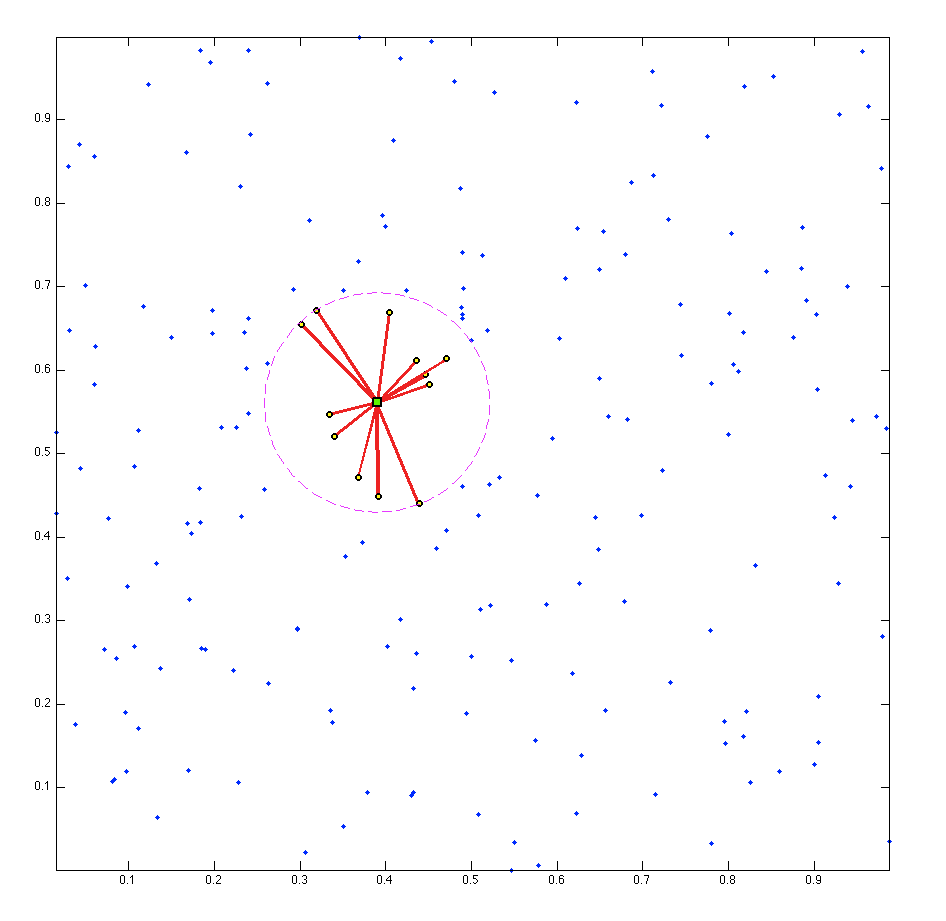
\includegraphics[width=1.0\textwidth]{../figures/chapter2/preview_stencils_example.png}
		\caption{A 13 node RBF-FD stencil of randomly distributed nodes. The stencil centered at the green square contains the 12 nearest neighbors contained within the minimum covering circle drawn in purple.}
		\label{fig:stencil_example_random}
	\end{subfigure}
	\begin{subfigure}[m]{0.35\textwidth}
		\centering
		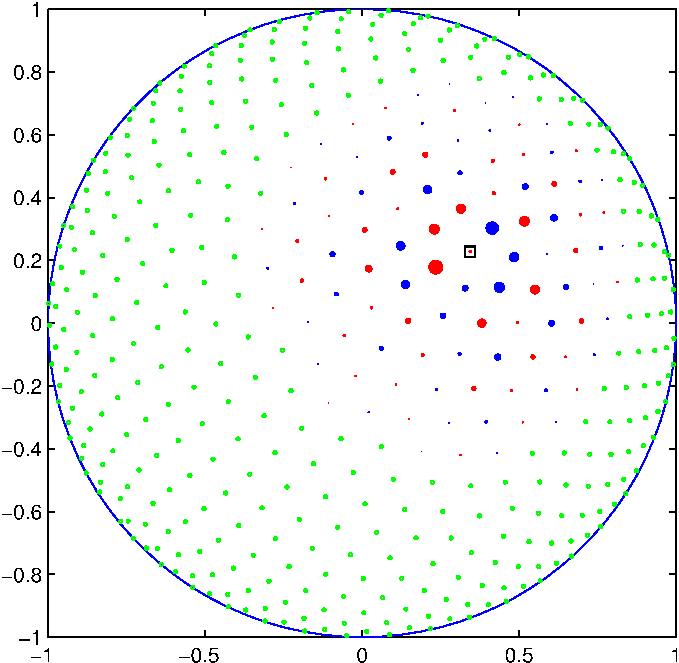
\includegraphics[width=1.0\textwidth]{../figures/chapter2/RBFFD_single-eps-converted-to.pdf}
		\caption{A 75 node RBF-FD stencil with blue (negative) and red (positive) differentiation weights to approximate advective operator at the square. Stencils weights indicated by scale of disk radii. (Image courtesy of Bengt Fornberg and Natasha Flyer)}
		\label{fig:stencil_example_sphere}
	\end{subfigure}
	\caption{Examples of stencils computable with RBF-FD \authnote{Consider: show example FD stencil (5pt with regular grid)}}
	\label{fig:stencil_example}
\end{figure}


\section{RBF-FD weights}
\label{sec:rbffd}

Given a set of function values, $\{u(\vx_j)\}_{j=1}^{N}$, on a set of $N$ nodes $\{\vx_j\}_{j=1}^{N}$, the operator $\diffop$ acting on $u(\vx)$ evaluated at 
$\vx_j$, %$u(\vx_j)$ 
is approximated by a weighted combination of function values, $\{u(\vx_i)\}_{i=1}^{n}$, in a small neighborhood of $\vx_j$, 
where $n\ll N$ defines the size of the stencil. 
%(added constant term to equation:)
\begin{align}
\diffop{u(\vx)}\mid_{\vx=\vx_j} &\approx \sum_{i=1}^{n} w_i u(\vx_i) + w_{n+1} p_0
\label{eq:derivFromFDWeights}
\end{align}
The RBF-FD weights, ${w_i}$, are found by enforcing that they are exact within the space spanned by the RBFs $\phi_i(\epsilon r) = \phi(\ep\vectornorm{\vx-\vx_{i}})$, centered at the nodes $\{\vx_i\}_{i=1}^{n}$, with 
$r=\vectornorm{\vx - \vx_i}$
being the distance between where the RBF is centered and where it is evaluated as measured in the standard Euclidean 2-norm. Various studies show  \cite{WrightFornberg06,FornbergDriscoll02,FornbergLehto11,FlyerLehto11} that better accuracy is achieved when the 
interpolant can exactly reproduce a constant, $p_0$.  
Assuming $p_0 = 1$, the constraint $\sum_{i=1}^{n}w_i=\diffop{1}|_{\vx=\vx_{j}}=0$ completes the system: 
%Address how the constraint is added. $w_{n+1}$ is mentioned without being defined.
%($\epsilon$ has been moved outside the norm on the RHS)
\begin{align}
\begin{pmatrix}
\phi(\epsilon\vectornorm{\vx_1-\vx_1}) & \phi(\epsilon\vectornorm{\vx_1-\vx_2} & \cdots & \phi(\epsilon\vectornorm{\vx_1-\vx_n}) & 1 \\
\phi(\epsilon\vectornorm{\vx_2-\vx_1}) & \phi(\epsilon\vectornorm{\vx_2-\vx_2} & \cdots &
\phi(\epsilon\vectornorm{\vx_2-\vx_n}) & 1\\
\vdots & \ddots & \ddots & \vdots & \vdots\\
\phi(\epsilon\vectornorm{\vx_n-\vx_1}) & \phi(\epsilon\vectornorm{\vx_n-\vx_2} & \cdots &
\phi(\epsilon\vectornorm{\vx_n-\vx_n}) & 1 \\
1 & 1 & \cdots & 1 & 0
\end{pmatrix}
\begin{bmatrix} w_1 \\ w_2 \\ \vdots \\ w_n  \\ w_{n+1}\end{bmatrix}
&=
\begin{bmatrix} \diffop{\phi(\ep\vectornorm{\vx-\vx_{1}})}|_{\vx=\vx_{j}} \\
                \diffop{\phi(\ep\vectornorm{\vx-\vx_{2}})}|_{\vx=\vx_{j}} \\ \vdots \\  \diffop{\phi(\ep\vectornorm{\vx-\vx_{n}})}|_{\vx=\vx_{j}}\\
                0
\end{bmatrix},
\label{eq:rbffd_weight_system}
\end{align}
where $w_{n+1}$ is ignored after the matrix in ({\ref{eq:rbffd_weight_system}}) is inverted.
This $n \times n$ system solve is repeated for each stencil center  $\vx_j$, $j=1...N$, to form the $N$ rows of the DM  with $n$ non-zeros $(n\ll N)$ per row.
As an example, if $\diffop$ is the identity operator, 
then the above procedure leads to RBF-FD interpolation. If $\diffop=\pd{}{x}$, one obtains the DM that approximates the first derivative in $x$. In the context of time-dependent PDEs,  the stencil weights remain constant for all time-steps when the nodes are stationary. Therefore, the calculation of the 
differentiation weights is performed once in a single preprocessing step of O$(n^3N)$ 
%floating point operations (FLOPs). 
FLOPs.
Improved efficiency is achieved
by processing multiple right hand sides in one pass, calculating the weights
corresponding to all required derivative quantities (i.e., $\pd{}{x}$, $\pd{}{y}$, $\Laplacian$, etc.).

%reply to the LSH question from the reviewer involving parallelization of the search process for each point, and the issue regarding embarrassingly parallel process. Also note: this is done only once so efficiency is not an issue, nor is parallelization.

For each of the $N$ small system solves of Equation~(\ref{eq:rbffd_weight_system}), the $n$ nearest neighbors to $\vx_j$ need to be located. This can be done efficiently using neighbor query algorithms or spatial partitioning data-structures such as Locality Sensitive Hashing (LSH) and $k$D-Tree. Different query algorithms often have a profound impact on the DM structure and memory access patterns. We choose a Raster ($ijk$) ordering LSH algorithm \cite{Bollig2011} leading to the matrix structure in Figures~\ref{fig:oneThreadPerStencil} and \ref{fig:oneWarpPerStencil}. While querying neighbors for each stencil is an embarrassingly parallel operation, the node sets used here are stationary and require stencil generation only once. Efficiency and parallelism for this task has little impact on the overall run-time of tests, which is dominated by the time-stepping. We preprocess node sets and generate stencils serially, then load stencils and nodes from disk at run-time. In contrast to the RBF-FD view of a static grid, Lagrangian/particle based PDE algorithms promote efficient parallel variants of LSH in order to accelerate querying neighbors at each time-step \cite{Pan2011, Goswami2010}. 


\section{Weight Operators}
Throughout the development of our parallel code we have verified code correctness through the solution of a variety of PDEs. Here we provide a list of operators we have tested and their corresponding equations for the RHS of Equation~\ref{eq:rbffd_weight_system} necessary to compute RBF-FD weights. 

The standard first derivatives $\pd{}{x}, \pd{}{y}, \pd{}{z}$ are produced by the chain rule
	\begin{align} 
	 \pd{\phi}{x} = \d{r}{x} \d{\phi}{r} = \frac{(x-x_{j})}{r} \d{\phi}{r} \\
	 \pd{\phi}{y} = \d{r}{y} \d{\phi}{r} = \frac{(y-y_{j})}{r} \d{\phi}{r} \\
	 \pd{\phi}{z} = \d{r}{z} \d{\phi}{r} = \frac{(z-z_{j})}{r} \d{\phi}{r}
	\end{align}

where $\pd{\phi}{r}$ for the Gaussian RBFs is given by: 


\subsection{Laplacian ($\Laplacian$)}

2D: 

3D: 

\subsection{Laplace-Beltrami ($\LaplaceBeltrami$) on the Sphere}

The $\Laplacian$ operator can be represented in spherical polar coordinates for $\mathbb{R}^3$ as: 
\begin{align} 
\Laplacian = \underbrace{\frac{1}{r} \pd{}{r} \left( r^{2} \pd{}{r}  \right)}_{\mathsf{radial}} + \underbrace{\frac{1}{r^2} \Delta_{S}}_{\mathsf{angular}} , \label{eq:laplacian_in_spherical}
\end{align}
where $\LaplaceBeltrami$ is the Laplace-Beltrami operator---i.e., the Laplacian operator constrained to the surface of the sphere. This form nicely illustrates the separation of components into radial and angular terms. 

In the case of PDEs solved on the unit sphere, there is no radial term, so we have:
\begin{align}
\Laplacian  \equiv \LaplaceBeltrami.
\end{align}
Although this originated in the spherical coordinate system, \cite{WrightFlyerYuen10} introduced the following Laplaci-Beltrami operator for the surface of the sphere: 
\begin{align} 
\LaplaceBeltrami = \frac{1}{4} \left[ \left(4-r^2\right) \pdd{}{r} + \frac{4-3r^2}{r} \pd{}{r} \right],
\end{align} 
where $r$ is the Euclidean distance between nodes of an RBF-FD stencil and is independent of our choice of coordinate system. 

\subsection{Constrained Gradient ($P_{x} \cdot \grad$) on the Sphere}

Additionally following \cite{FlyerWright09, FlyerLehto11}, the gradient operator must also be constrained to the sphere with this projection matrix: 
%\frac{1}{||\mathbf{x}||}
\begin{align}
P = I - \mathbf{x} \mathbf{x}^T =  \begin{pmatrix} 
(1-x_1^2) & -x_1 x_2 & -x_1 x_3 \\
-x_1 x_2 & (1-x_2^2) & -x_2 x_3 \\ 
-x_1 x_3 & -x_2 x_3 & (1-x_3^2) 
\end{pmatrix} = \begin{pmatrix} P_{x_1} \\ P_{x_2} \\ P_{x_3} \end{pmatrix}
\label{eq:project_gradient}
\end{align}
where $\mathbf{x}$ is the unit normal at the stencil center. 


The direct method of computing RBF-FD weights for the projected gradient for $\mathbf{P} \cdot \nabla $ is presented in \cite{FlyerWright09}. When solving for the weights, we apply the projection on the right hand side of our small linear system. We let $\vx = \begin{pmatrix} x_1, x_2, x_3 \end{pmatrix} $ be the stencil center, and $\vx_k=\begin{pmatrix} x_{1,k}, x_{2,k}, x_{3,k}\end{pmatrix}$ indicate an RBF-FD stencil node. 

Using the chain rule, and assumption that 
$$r(\vx_k-\vx)=\vectornorm{\vx_k-\vx} = \sqrt{(x_{1,k}-x_1)^2 + (x_{2,k}-x_2)^2 + (x_{3,k}-x_3)^2},$$
 we obtain the unprojected gradient of $\phi$ as
$$\nabla \phi(r(\vx_k - \vx)) = \pd{r}{\vx} \pd{\phi(r(\vx_k - \vx))}{r} = - (\vx_k - \vx)\frac{1}{r(\vx_k - \vx)} \pd{\phi(r(\vx_k - \vx))}{r}$$. 

Applying the projection matrix gives 
\begin{align*}
\mathbf{P} \nabla \phi(r(\vx_k - \vx)) & = - (\mathbf{P} \cdot \vx_k - \mathbf{P}\cdot\vx)\frac{1}{r(\vx_k - \vx)} \pd{\phi(r(\vx_k - \vx))}{r} \\
& =  - (\mathbf{P}\cdot\vx_k - 0)\frac{1}{r(\vx_k - \vx)} \pd{\phi(r(\vx_k - \vx))}{r} \\
& = - (I-\vx\vx^T)(\vx_k
)\frac{1}{r(\vx_k - \vx)} \pd{\phi(r(\vx_k - \vx))}{r} \\
& = \begin{pmatrix} x \vx^T \vx_k - x_k \\ y \vx^T \vx_k -  y_k \\ z \vx^T \vx_k -z_k \end{pmatrix} \frac{1}{r(\vx_k - \vx)} \pd{\phi(r(\vx_k - \vx))}{r} 
 \end{align*}
Thus, we directly compute the weights for $P_{x}\cdot\grad{}$ using these three RHS in Equation~\ref{eq:rbffd_weight_system}: 
\begin{align} 
P\pd{}{x_1} = ( x_1 \vx^T \vx_k - x_{1,k}) \frac{1}{r(\vx_k - \vx)} \pd{\phi(r(\vx_k - \vx))}{r} |_{\vx=\vx_j} \\
P\pd{}{x_2} = ( x_2 \vx^T \vx_k - x_{2,k}) \frac{1}{r(\vx_k - \vx)} \pd{\phi(r(\vx_k - \vx))}{r} |_{\vx=\vx_j} \\
P\pd{}{x_3} = ( x_3 \vx^T \vx_k - x_{3,k}) \frac{1}{r(\vx_k - \vx)} \pd{\phi(r(\vx_k - \vx))}{r} |_{\vx=\vx_j}
\end{align}

Alternatively, assuming weights for operators $\grad = \pd{}{x_{1}}, \pd{}{x_{2}}, \pd{}{x_{3}}$ are already computed, the projected operator could be constructed via weighting the unprojected gradient components. For example: 

\authnote{Show accuracy of derivative approximation when using projected operator vs linear combinations of dx,dy,dz operators}


\section{Stabilization: Hyperviscosity}

For RBF-FD, differentiation matrices encode convective operators of the form 
\begin{equation}
D = \alpha \pd{}{\lambda} + \beta \pd{}{\theta} \label{eqconv}
\end{equation}
where $\alpha$ and $\beta$ are a function of the fluid velocity. The convective operator, discretized
through RBF-FD, has eigenvalues 
%given 
 in the right half-plane causing the method to be unstable~\cite{FornbergLehto11, FlyerLehto11}. 
%. 
%Shorter previous sentence. What diff operator is being discretized by DM?
Stabilization of the RBF-FD method is achieved through the application of a hyperviscosity filter 
to Equation~(\ref{eqconv}) \cite{FornbergLehto11}. By using Gaussian 
 RBFs, $\phi(r) = e^{-(\epsilon r)^2}$, the hyperviscosity (a high order Laplacian operator) simplifies to
\begin{equation}
\Delta^{k}\phi(r) = \epsilon^{2k} p_k(r) \phi(r)
\label{eqn:gaussian_hv}
\end{equation}
where $k$ is the order of the Laplacian and  $p_k(r)$ are multiples of generalized Laguerre polynomials that
are generated recursively (see \cite{FornbergLehto11}: Section 3.2). We assume a 2D  Laplacian operator 
when working on the surface of the sphere since a local stencil can be viewed as lying on a plane.
%Since the purpose of hyperviscosity is to suppress the highly oscillatory modes while leaving all the smooth ones intact, it suffices to ignore the local curvature of the sphere, and calculate $\Delta^{k}\phi(r)$ as if the RBF-FD stencil was located on a 2D flat plane.
%A 2D approximation for the hyperviscosity suffices because its only role is to suppress spurious unphysical modes. The scale of hyperviscosity, on the order of $10^{-30}$, makes this a completely harmless assumption even in the case when the stencil radius is large relative to the size of the sphere.

%I do not understand question 2.8

In the case of parabolic and hyperbolic PDEs, hyperviscosity is added as a filter to the right hand side of the evaluation. For example, at the continuous level, 
the equation solved takes the form
\begin{equation}
\pd{u}{t} = - D u + H u,
\label{eq:evaluation_with_hyperviscosity}
\end{equation}
%Address the issue of continuous versus discrete form. Use words operator and matrix properly. \authnote{Double check}
where $D$ is the PDE operator, and $H$ is the hyperviscosity filter operator.
Applying hyperviscosity shifts all the eigenvalues of D to the left half of the complex plane. 
This shift is controlled by $k$, the order of the Laplacian, and a scaling parameter $\gamma_c$, defined by
\begin{equation*}	
H = \gamma \Delta^{k} = \gamma_c N^{-k} \Delta^{k}.
\end{equation*}
Given a choice of $\epsilon$ (see Section~\ref{sec:numerical_validation}), it was found experimentally that $\gamma = \gamma_c N^{-k}$  provides stability and good accuracy for all values of $N$ considered here. It also ensures that the viscosity vanishes as $N\rightarrow\infty$ \cite{FlyerLehto11}.
In general, the larger the stencil size, the higher the order of the Laplacian.  This is attributed to the fact that, for convective operators, larger stencils treat a wider range of modes accurately. As a result, the hyperviscosity operator should preserve as much of that range as possible. The parameter $\gamma_c$ must also be chosen with care and its sign depends on $k$ (for $k$ even, $\gamma_c$ will be negative and for $k$ odd, it will be positive). If $\gamma_c$ is too large, the eigenvalues move outside the stability domain of our time-stepping scheme and/or eigenvalues corresponding to lower physical modes are not left intact, reducing the accuracy of our approximation. If $\gamma_c$ is too small, eigenvalues remain in the right half-plane \cite{FornbergLehto11,FlyerLehto11}.



% TODO: Break off to new chapter
\chapter{TEMP}


\section{Fragments (integrate above)}

Stabilization of the RBF-FD method is achieved through the application of a hyperviscosity filter \cite{Fornberg2011b}. By assuming the use of Gaussian RBFs, $\phi(r) = e^{-(\epsilon r)^2}$, the hyperviscosity operator simplifies to
\begin{equation}
\Delta^{k}\phi(r) = \epsilon^{2k} p_k(r) \phi(r).
\label{eqn:gaussian_hv}
\end{equation}
The multiples of generalized Laguerre polynomials, $p_k(r)$, are obtained through the following recursive relation:
\begin{align*}
\begin{cases} 
p_0(r) &=1, \\
p_1(r) &= 4(\epsilon r)^2 - 2d, \\
p_k(r) &= 4((\epsilon r)^2 - 2(k-1) - \frac{d}{2})  p_{k-1}(r) - 8(k-1)(2(k-1) - 2 + d) p_{k-2}(r), \ \ \ \ k = 2, 3, ...
\end{cases}
\end{align*}
where $d$ is the dimension of the problem. We assume $d=2$ below when working on the surface of the sphere.


Many algorithms exist to query the $k$-nearest neighbors (equivalently all nodes in the minimum/smallest enclosing circle). Some algorithms overlay a grid similar to Locality Sensitive Hashing and query such as... \cite{HarPeledMazumdar2003}.


\subsubsection{Conditioning} 
Conditioning is defined as: 

With condition number estimates we can choose a proper support parameter for uniformly distributed node sets.

Alternative algorithms exist for solving for RBF-FD weights when the systems are overly ill-conditioned. Currently, we have an unpublished algorithm ContourSVD available to play with (demonstrate accuracy improvements). 

\subsubsection{Node Placement -- Centroidal Voronoi Tessellation}
We make the assumption for now that we use regularly distributed nodes. Centroidal Voronoi tessellations provide reasonably good distributions for solutions. Examples (heat ellipse, ellipsoid, sphere, square cavity).

The motivation behind RBF-FD is generality/functionality in the numerical method. Scattered nodes are supported. Distribution requires proper choice of support, and tight nodes result in increased conditioning

\section{Approximate Nearest Neighbor (ANN) Query}

RBF methods are traditionally described as general and meshless in that they apply to unstructured clouds of points in arbitrary dimensions. However, although the term meshless implies a method capable of operating with no node connectivity, all numerical methods---meshless RBF methods included---connect nodes in the domain. For example, the ``meshless'' global RBF method connects every node in the domain to all other nodes. Compact support or local RBF methods like RBF-FD limit connections to nodes that lie within a predetermined radius.

The connections between nodes form a directed adjacency graph with edges that dictate the paths along which data/phenomena can travel. For example, a plus shaped stencil of five points with a center node and four neighboring nodes allows values to propagate north, south, east and west; not northeast, southeast, etc.


They are robust and function on scattered point clouds. RBF-FD in particular requires stencils to be generated from $n$ nearest neighbors to a stencil center. The cost of these neighbor queries can vary greatly depending on the choice of algorithm or data-structure used to make the query. 

For example, in general brute force is inefficient 
The author of \cite{Fasshauer2007} queries $n$ nearest neighbors for a compact-support RBF partition of unity example with a $k$-D tree. In \cite{FlyerLehto11,FornbergLehto11} a $k$-D Tree is leveraged for all neighbor queries for RBF-FD. 

In our work in \cite{BolligFlyerErlebacher2012} an alternative to $k$-D tree was leveraged, based loosely on Locality Sensitive Hashing.

\subsection{$k$-D Tree}

Most of the RBF community leverages the $k$-D tree, due to its low computational complexity for querying neighbors and its wide availability as standalone software in the public domain (e.g., matlab central has a few implementations for download, and the MATLAB Statistics Toolbox includes an efficient k-D Tree). 

The complexity of assembling he tree is

The Matlab central $k$-D Tree is MEX compiled and efficient. We integrated the standalone C++ code into our library.  

While the $k$-D Tree functions well for queries, its downfall is a large cost in preprocessing to build the tree. For moving nodes, such as in Lagrangian schemes, this cost is prohibitively high. In an attempt to reduce the cost, lagrangian schemes introduced approximate nearest neighbor queries based on 

Approximate nearest neighbors will be nearly balanced. 
We observe that RBF-FD functions as well on stencils of true nearest neighbors as it does on approximate nearest neighbors. 


\ifstandalone
\bibliographystyle{plain}
\bibliography{merged_references}
\end{document}
\else
\expandafter\endinput
\fi

